\chapter{Reflexionsseismik}
In diesem Kapitel wollen wir uns mit einer weiteren geophysikalischen Messmethode aus dem Gebiet der Seismik beschäftigen. Diese Methode nutzt wie die Refraktionsseismik künstlich erzeugte seismische Wellen, wertet aber hauptsächlich die reflektierten Wellen aus. Das Hauptziel einer reflexionsseismischen Messung ist die Lokalisierung von Schichtgrenzen.

Typisch für die Reflexionsseismik ist die riesige Datenmenge, die bei der Messung aufgenommen wird, da die Profillänge meist mehrere zehn Kilometer lang ist. Diese Datenmengen sorgen für eine geringe Mehrdeutigkeit in der Auswertung und macht die Reflexionsseismik damit zur geophysikalischen Messmethode mit der zuverlässigsten Aussage über den Untergrund. Allerdings ist der Kostenaufwand einer solchen Messung enorm hoch. Weiterhin ist die Datenverarbeitung aus Datenauswertung sehr aufwändig und erfordert High-Performance-Computing. 


Die Eindringtiefe liegt in der Regel zwischen 100\,m und 1\,km. Tiefenseismische Messungen dringen jedoch in Tiefen bis zu 100\,km vor.   

Anwendung findet die Reflexionsseismik in Forschungsbereichen zur Rohstoffexploration, Energiegewinnung und Endlagerung.


\section{Zero-Offset-Konfiguration}
Dies ist die einfachste Messkonfiguration für eine reflexionsseismische Messung. Sender um Empfänger stehen hier am gleichen Ort.

\begin{figure}[H]
	\centering
	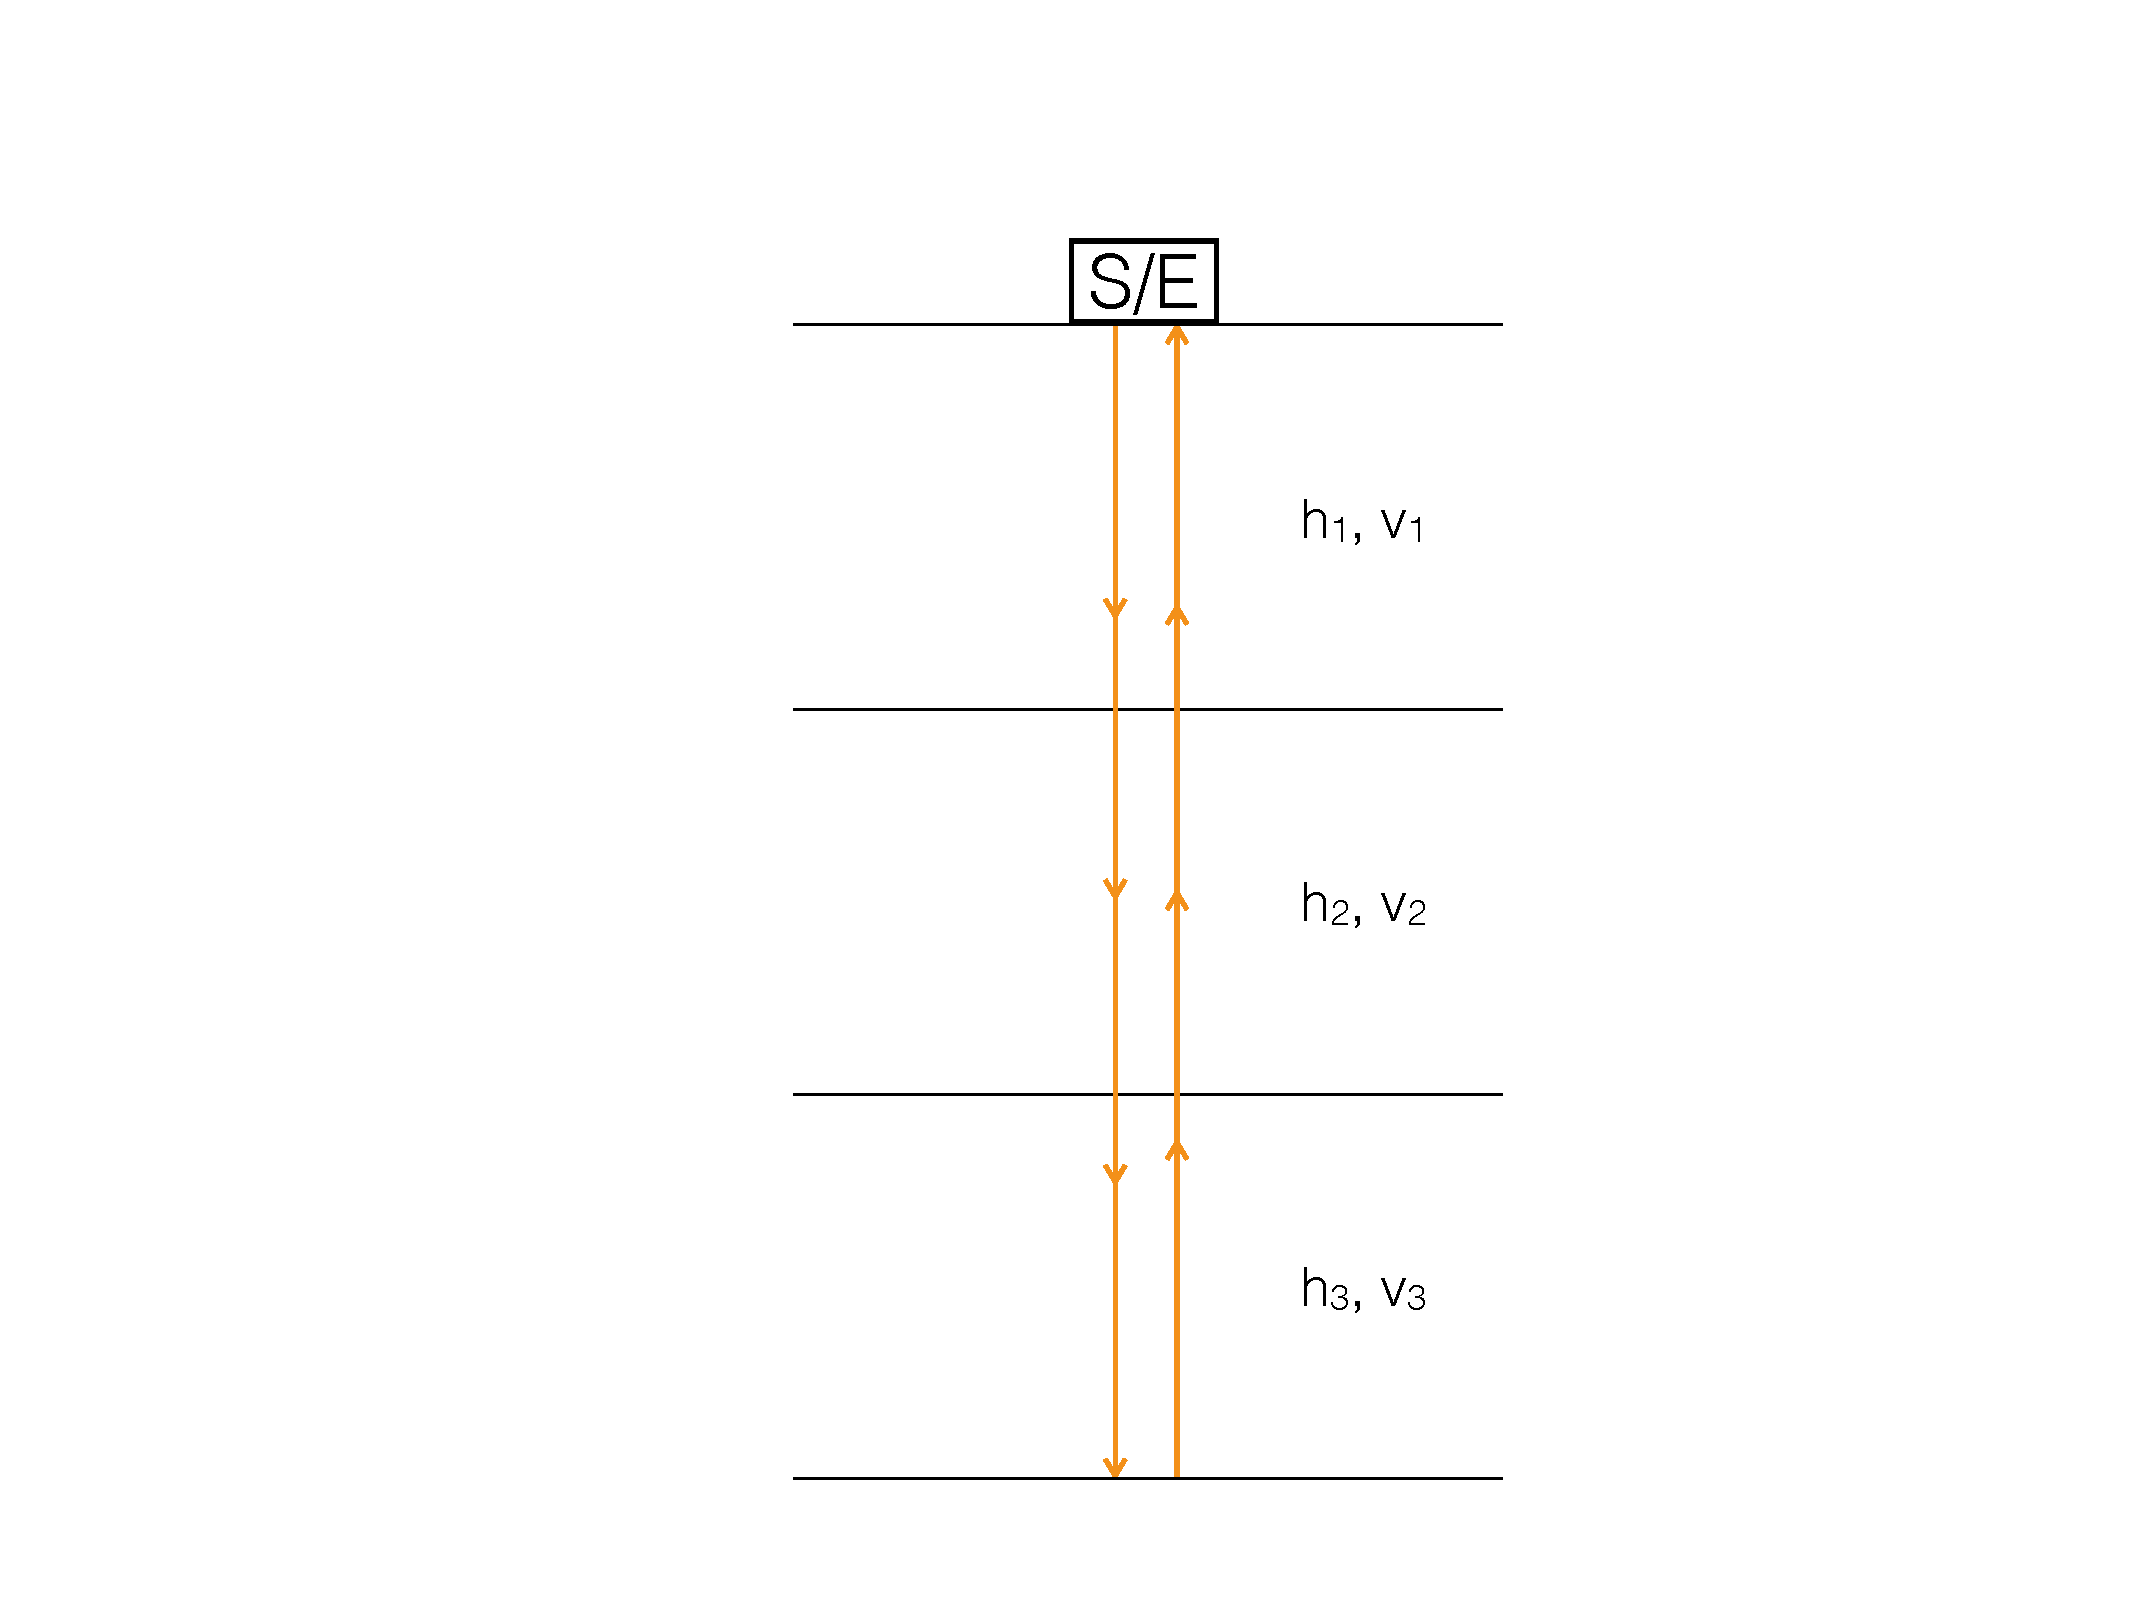
\includegraphics[scale = 0.3]{ReflexionsseismikBilder/ZeroOffset}
\end{figure}


Allerdings hat diese Methode einige \textbf{Probleme}: \begin{itemize}
	\item sehr anfällig für Verzerrungen: Laufzeiten entsprechen nicht Reflektortiefen
	\item schlechtes Signal-/Stör-Verhältnis: jeder Punkt im Untergrund wird nur einmal beleuchtet
	\item große Mehrdeutigkeiten
\end{itemize}

Durch Variation der Entfernung zwischen Sender und Empfänger, sowie einer Mehrfachabdeckung der Untergrundpunkte bei der Messung und Bestimmung des Geschwindigkeitsmodells, kann man diese Probleme lösen. Wie genau diese Messkonfiguration dann aussieht, und wie sie ausgewertet wird schauen wir uns im Folgenden an.

\section{Common-Midpoint-Technik}
Die Idee hinter dieser Methodik ist die Erweiterung eines Einzel-Offsets zu Multi-Offsets. Das bedeutet, dass wir alle Untergrundpunkte mehrfach durch Messungen abdecken. 

Unser Messaufbau sieht dann in etwa so aus: 

\begin{figure}[H]
	\centering
	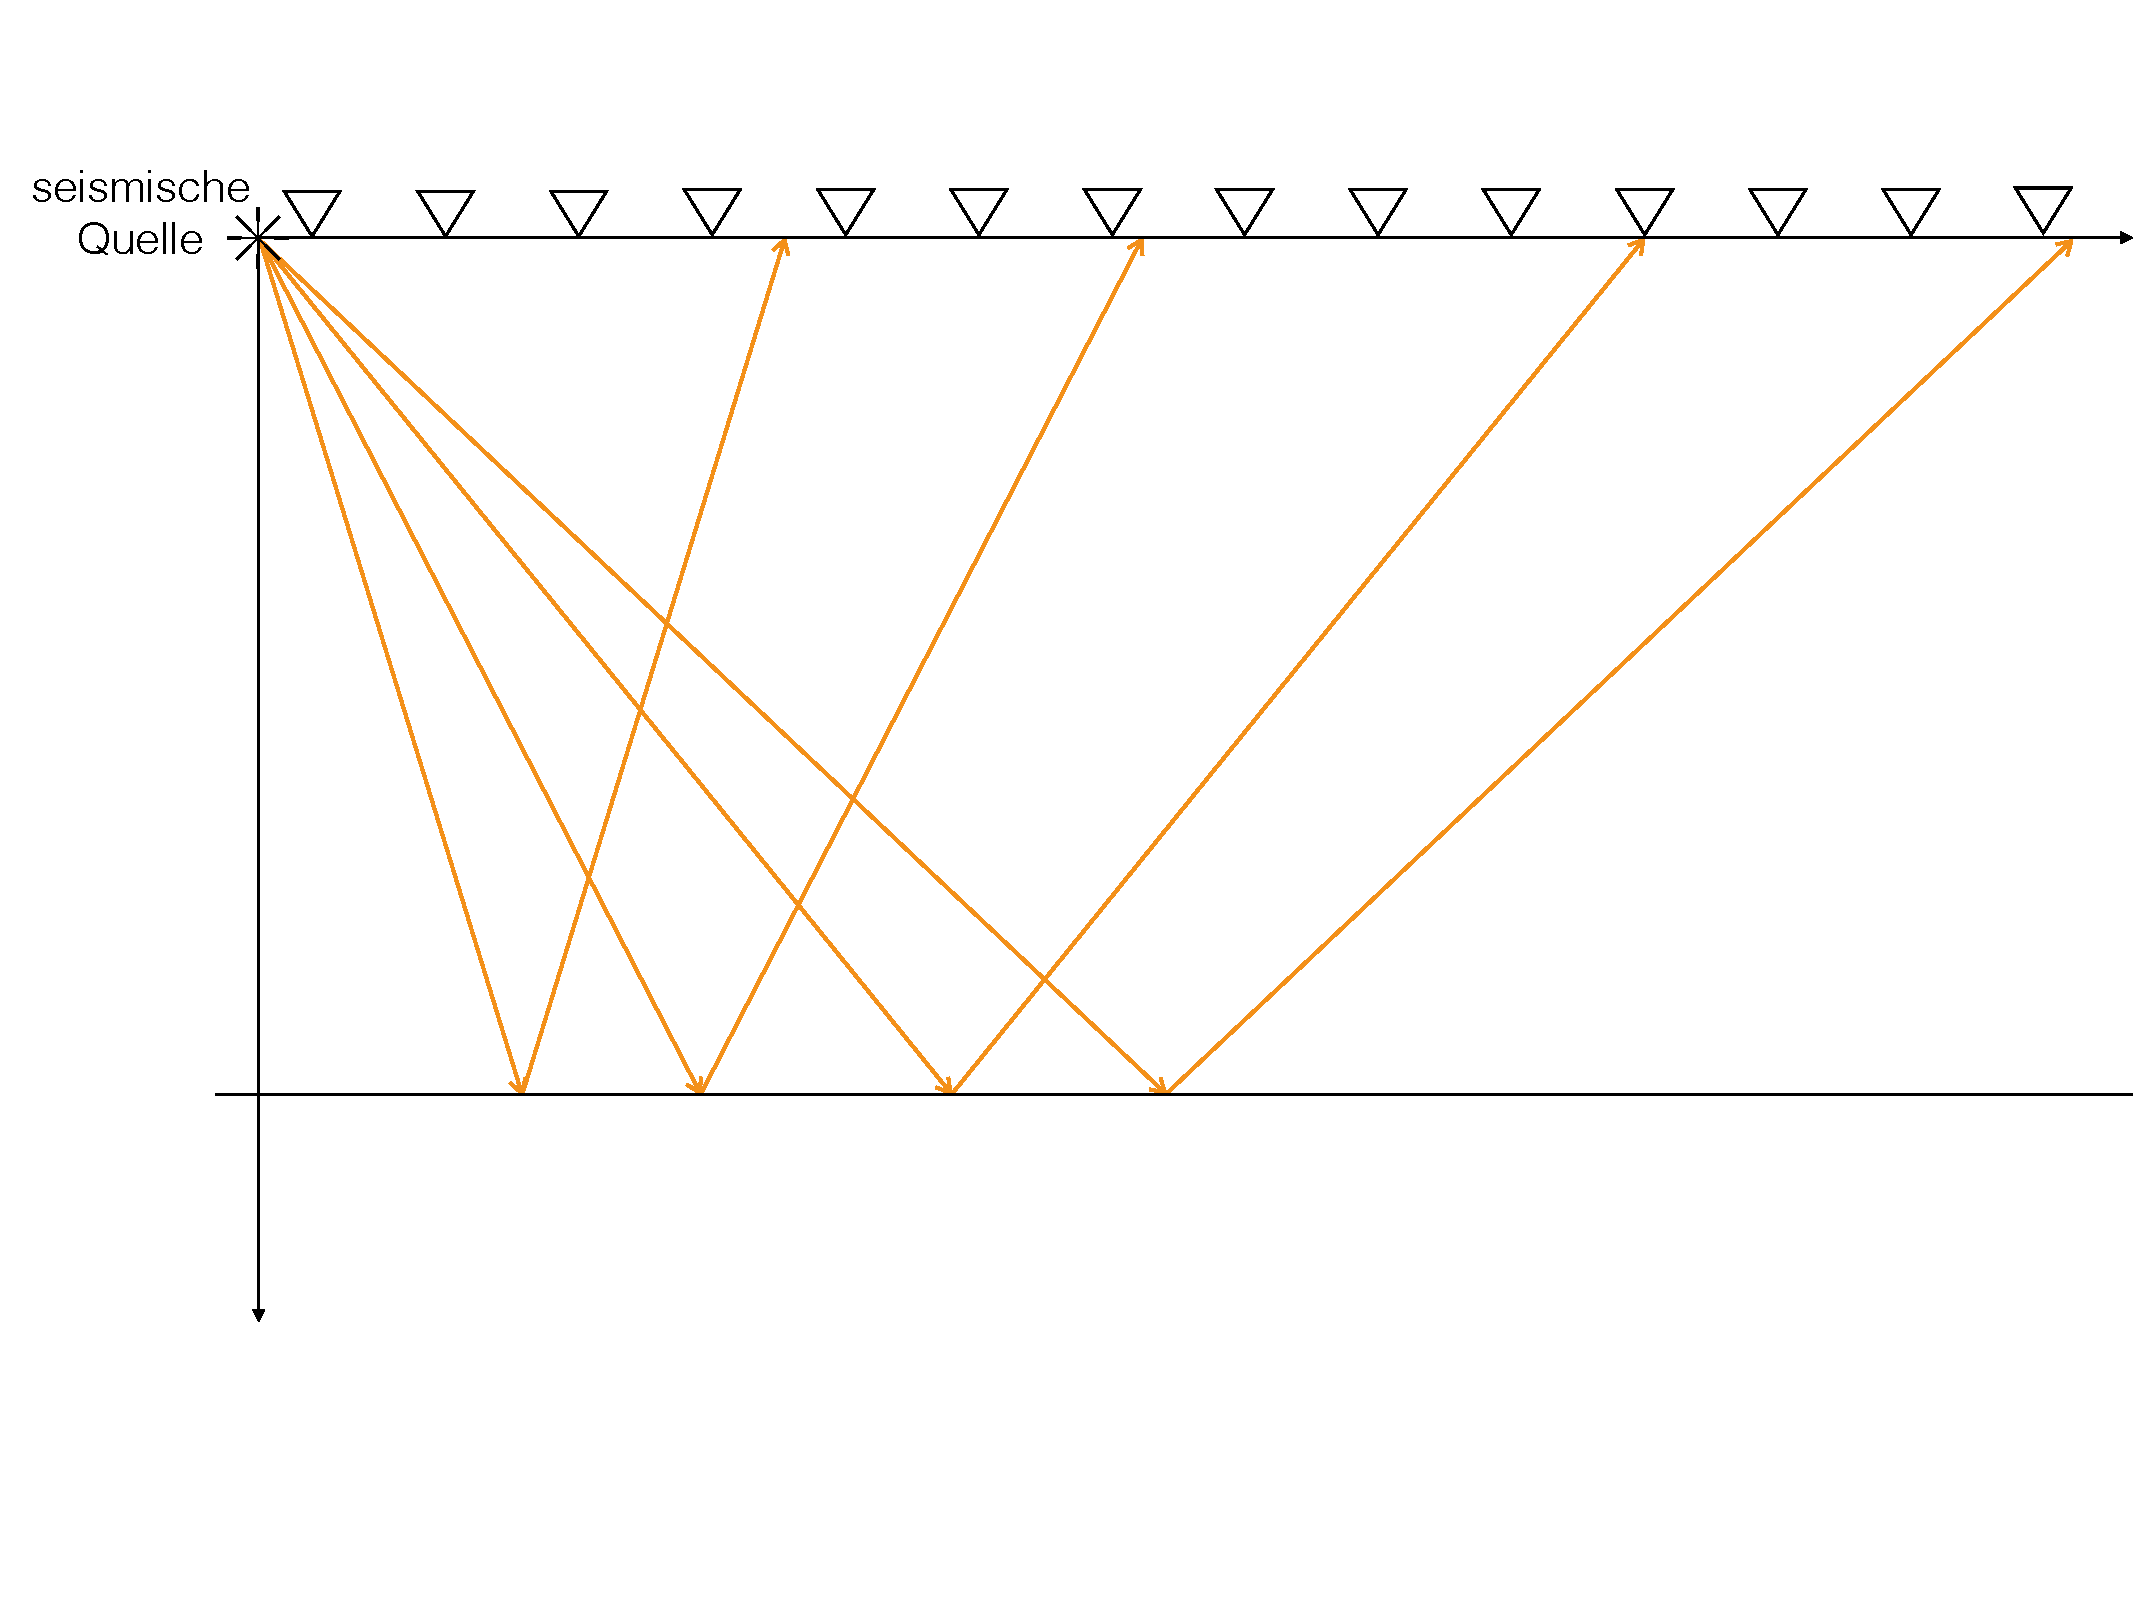
\includegraphics[width = \textwidth]{ReflexionsseismikBilder/MultiOffsetAnordnung}
\end{figure}


Im Wesentlichen besteht diese Messmethode aus fünf Arbeitsschritten: \begin{enumerate}[label={(\arabic*)}]
	\item Sortierung der Messpaare nach gemeinsamen Mittelpunkten (CMP)
	\item Geschwindigkeitsanalyse (Bestimmung von $v_{\text{nmo}}$)
	\item Laufzeitkorrektur
	\item Stapelung (Summation)
	\item Berechnung der Schichtgeschwindigkeiten
\end{enumerate}

Die einzelnen Arbeitsschritte werden im Folgenden erklärt.


\subsection{Sortierung nach CMP}
Der erste Schritt zur Auswertung ist die Sortierung der Messergebnisse nach einem gemeinsamen Mittelpunkt zwischen Quelle und Empfänger. Die so nach gemeinsamen Reflexionspunkt im Untergrund sortierten Seismogramme bilden einen \textbf{Common-Midpoint} (CMP). Liegt eine horizontale Schichtgrenze vor, liegt bei allen Messpaaren der Reflexionspunkt genau in der Mitte $x/2$ zwischen Sender und Empfänger (mit $x$ als Abstand Sender-Empfänger).

\begin{figure}[H]
	\centering
	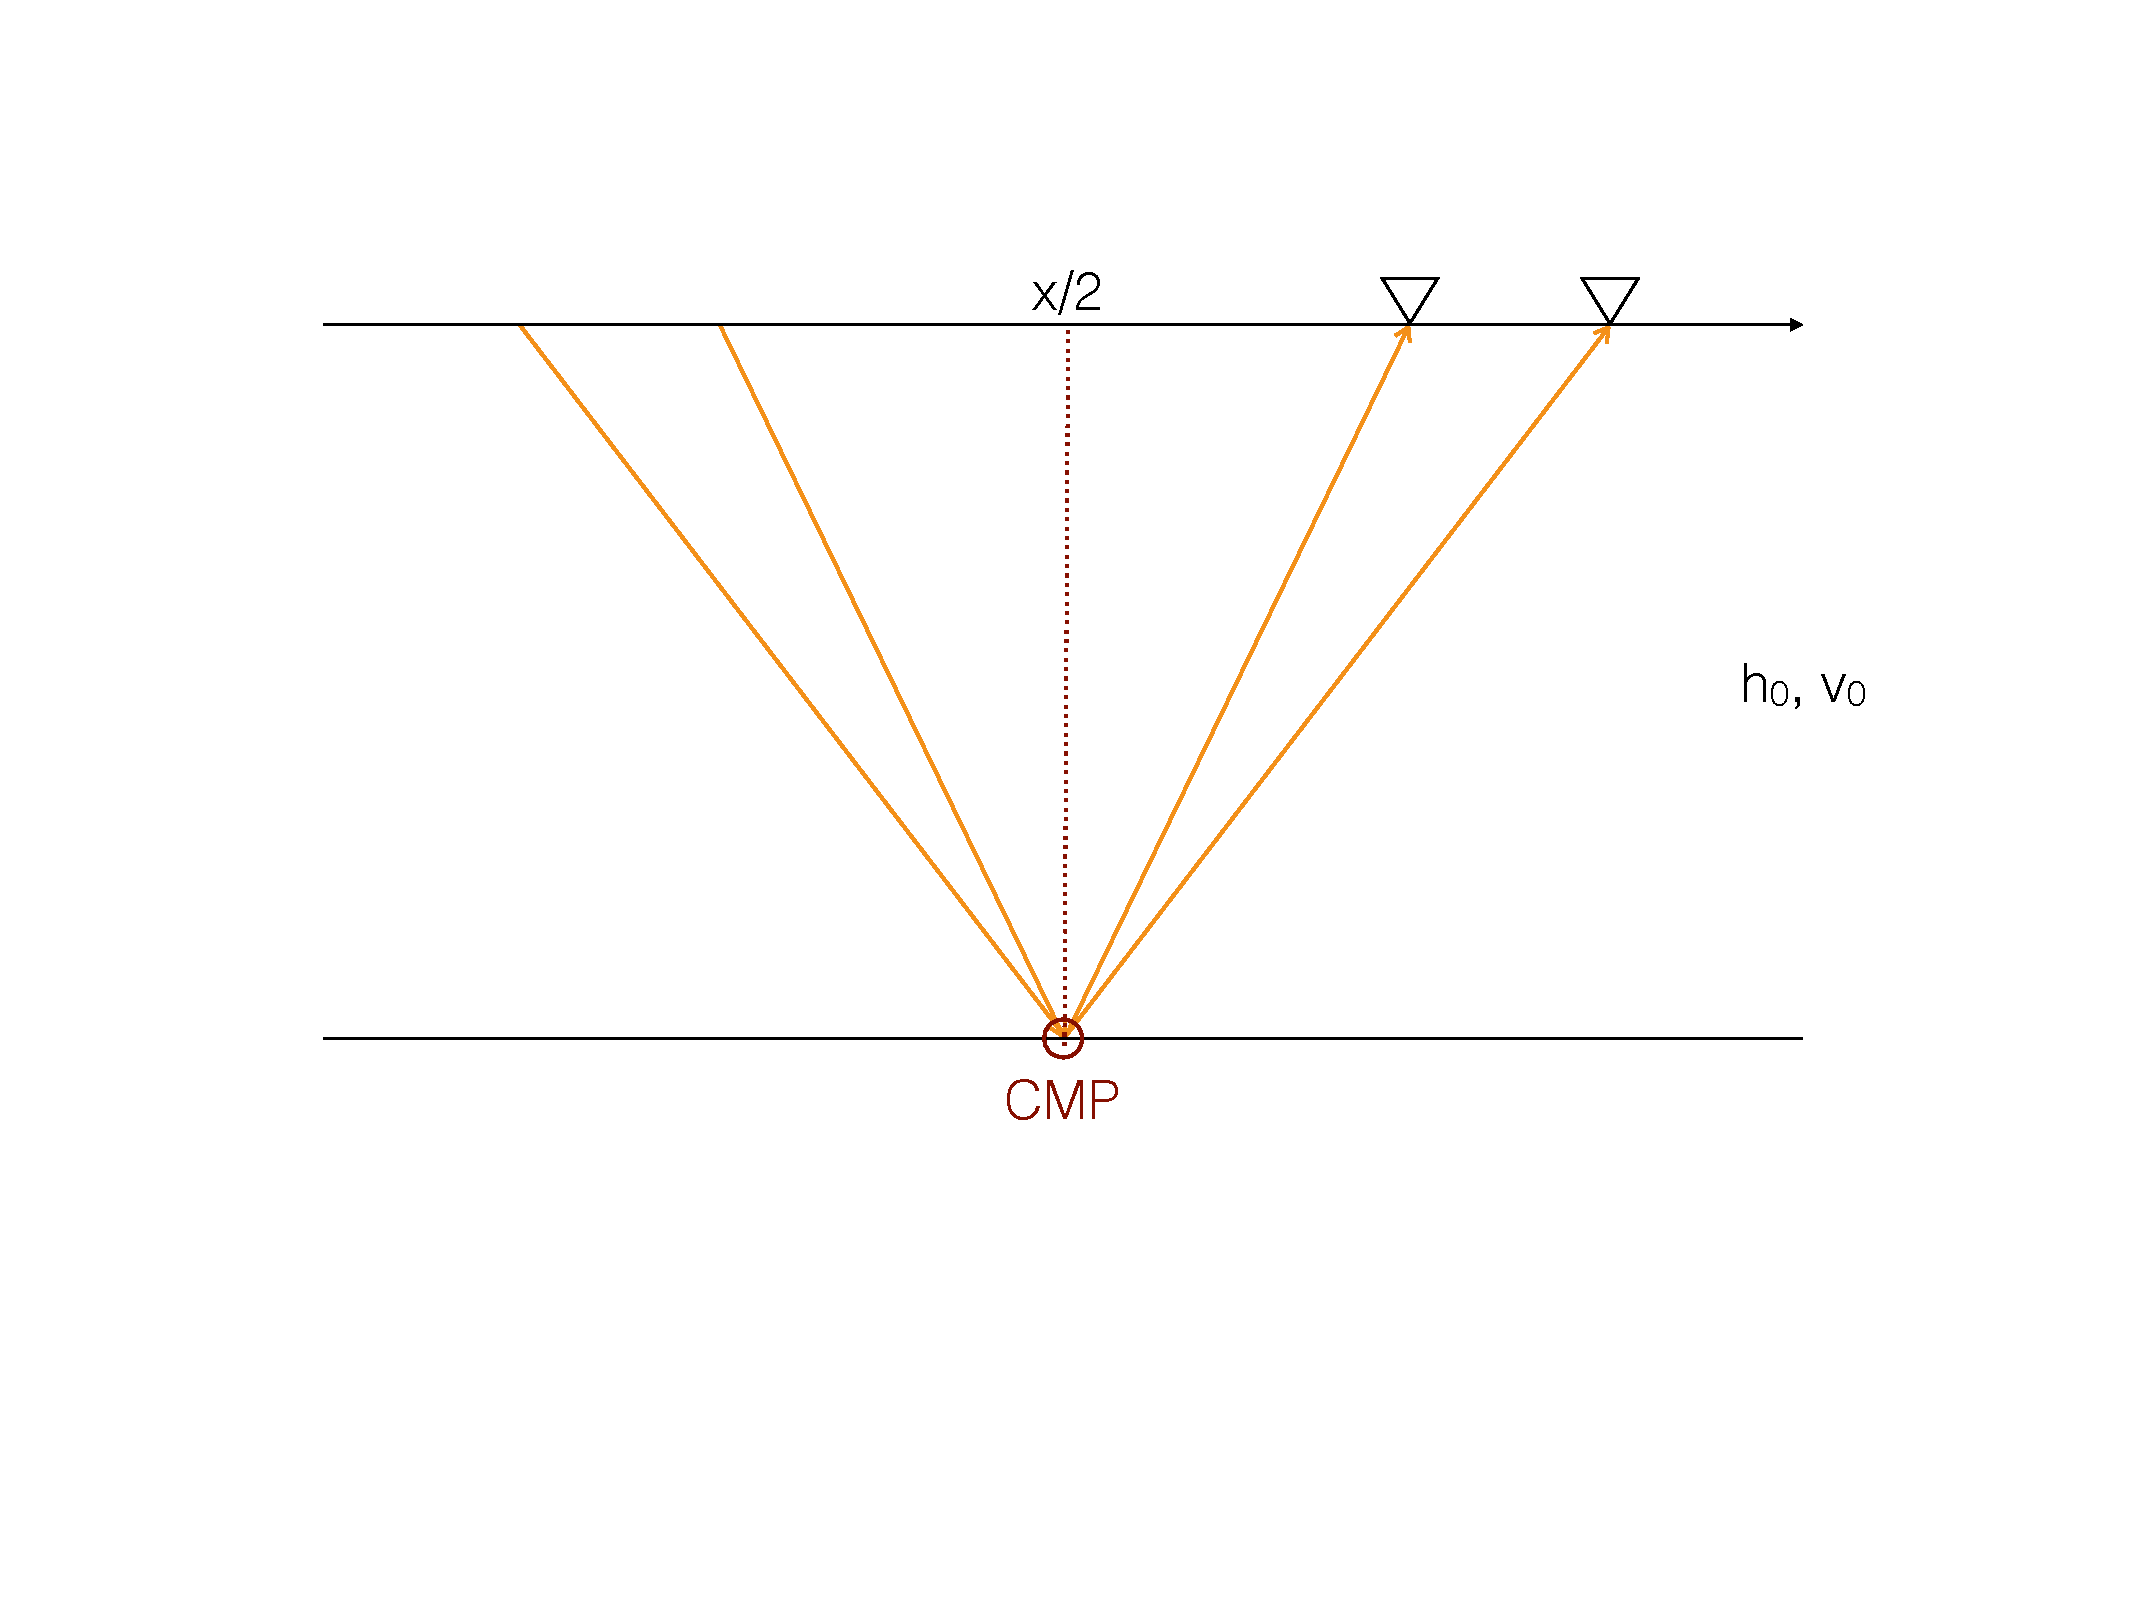
\includegraphics[width = \textwidth]{ReflexionsseismikBilder/CMPSortierung}
\end{figure}

\subsection{Laufzeitdiagramm und Geschwindigkeitsanalyse}
Wie auch schon bei der Refraktionsseismik interessieren wir uns besonders für die Ausbreitungsgeschwindigkeiten seismischer Wellen in allen Schichten. Um diese zu berechnen und zu analysieren, übertragen wir zunächst unsere gemessenen Werte in ein Laufzeitdiagramm. 

\begin{figure}[H]
	\centering
	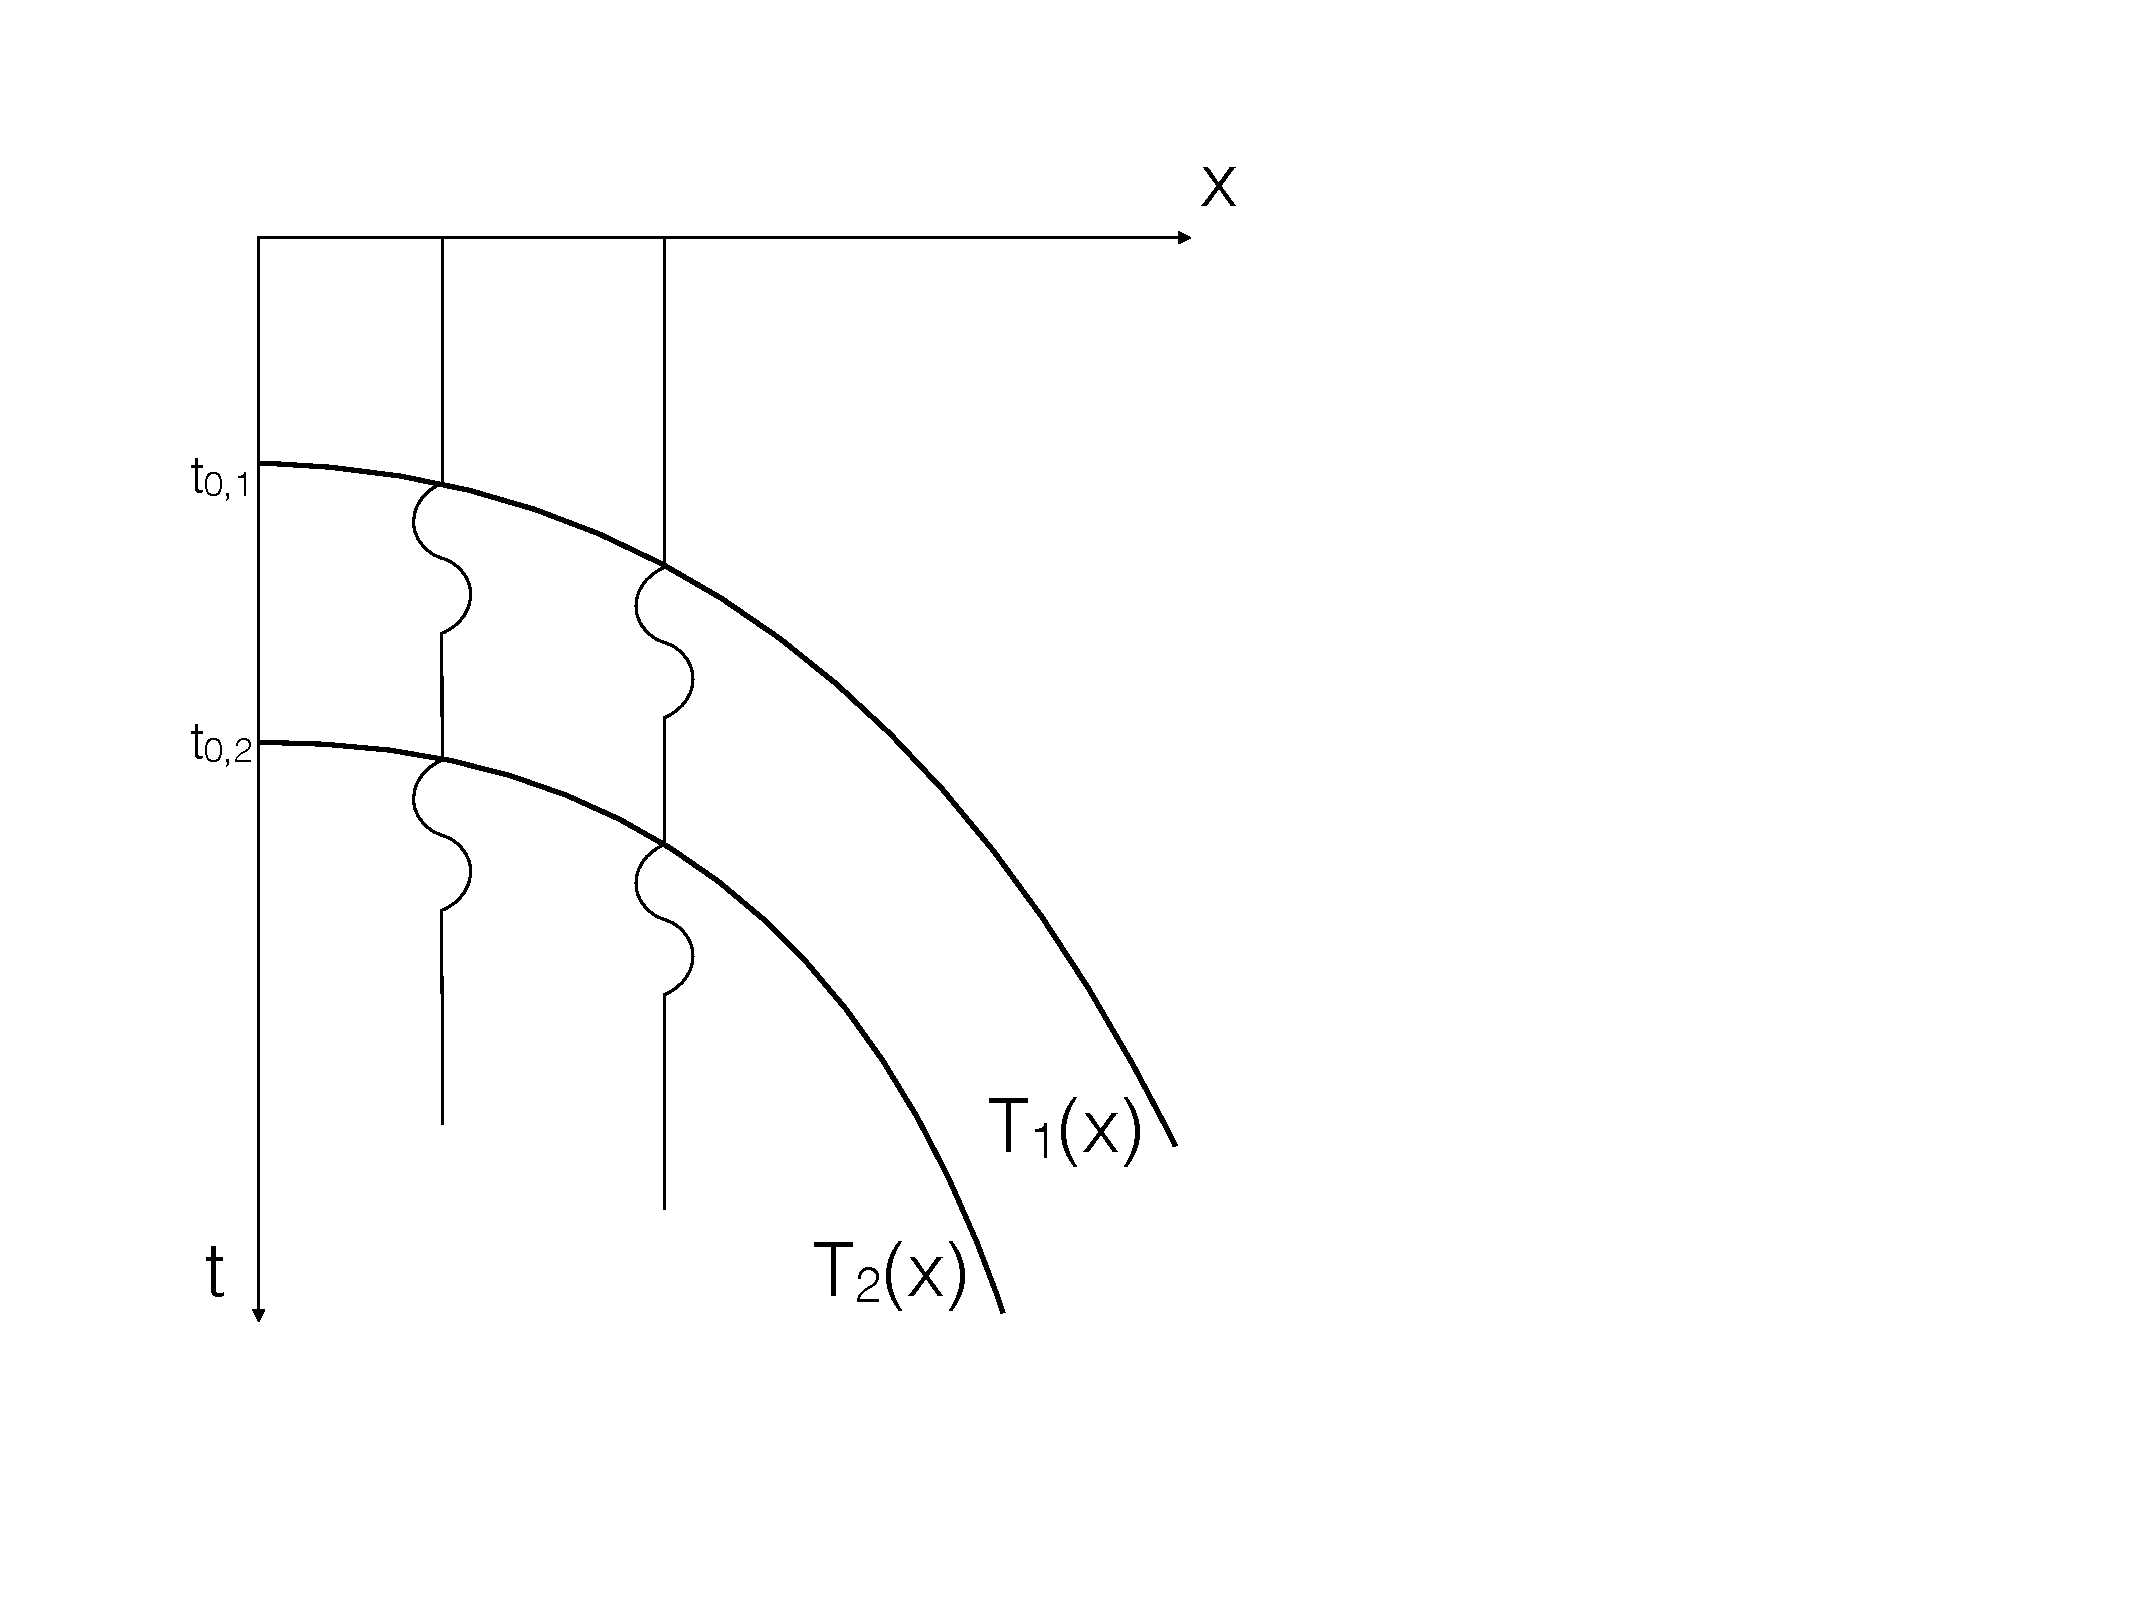
\includegraphics[scale = 0.3]{ReflexionsseismikBilder/t-x-Diagramm}
\end{figure} 


Die zugehörige Laufzeitgleichung ist nach Pythagoras: \begin{equation*}
	T^2(x) = \frac{x^2}{v_0^2} + t_0^2
\end{equation*}

Da diese Laufzeitgleichung eine Hyperbel ist, kann man die Geschwindigkeiten nicht einfach anhand der Steigung der Laufzeitkurve ablesen. Betrachtet man die Gleichung jedoch genauer, liegt nahe, die Messwerte in ein $T^2/ x^2$-Diagramm zu übertragen.

\begin{figure}[H]
	\centering
	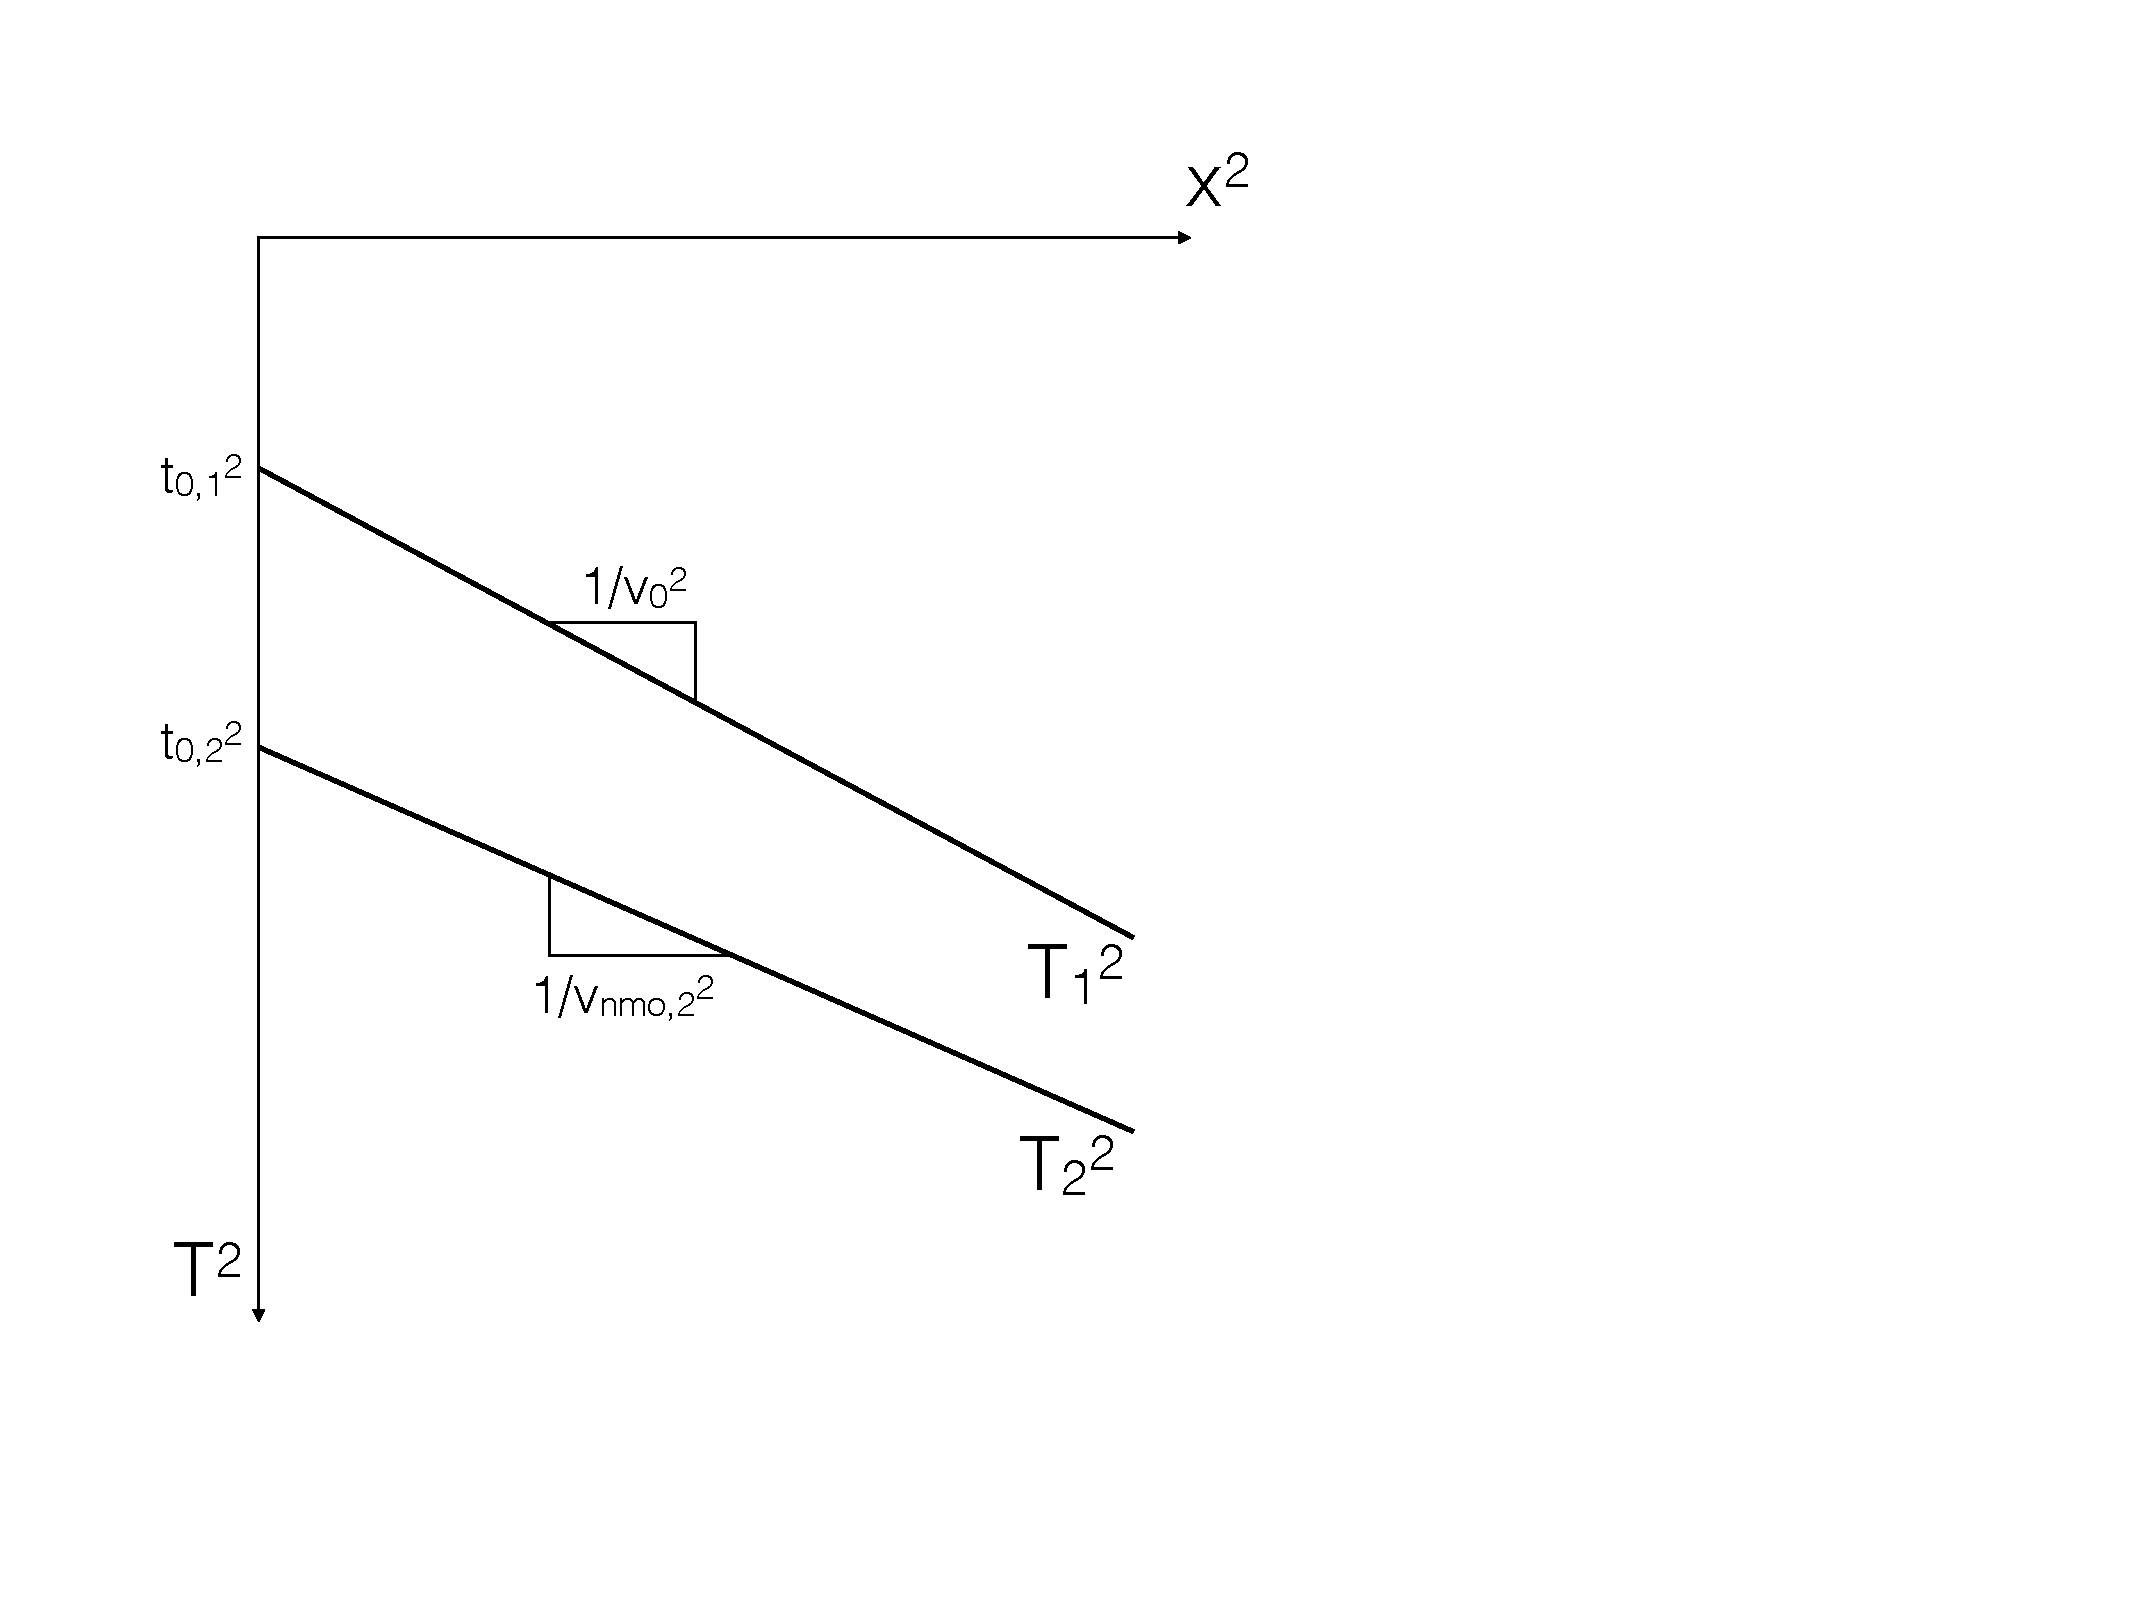
\includegraphics[scale = 0.3]{ReflexionsseismikBilder/T2-X2-Diagramm}
\end{figure}


An diesen Kurven könnte man nun die Geschwindigkeiten ablesen. Allerdings ist $T^2$ nur für die erste Schicht eine exakte Berechnung. Für alle weiteren ist sie nur eine Näherung. Die Geschwindigkeit, die man nach Berechnung der Steigung erhält, ist die \textbf{Normal-Moveout-Geschwindigkeit} $v_{\text{nmo}}$. Diese gibt lediglich die durchschnittliche Geschwindigkeit über alle Schichten an. \begin{align*}
	T_1^2(x) &= \frac{x^2}{v_1^2} + t_{0,1}^2 \\
	T_2^2(x) &\approx \frac{x^2}{v_{\text{nmo},2}^2} + t_{0,2}^2
\end{align*}

\subsection{Laufzeitkorrektur}
Das Ziel der CMP-Methode ist die Simulation einer Zero-Offset-Anordnung mit eindeutigen Ergebnissen durch mehrfache Abdeckung eines Untergrundpunktes. 

\begin{figure}[H]
	\centering
	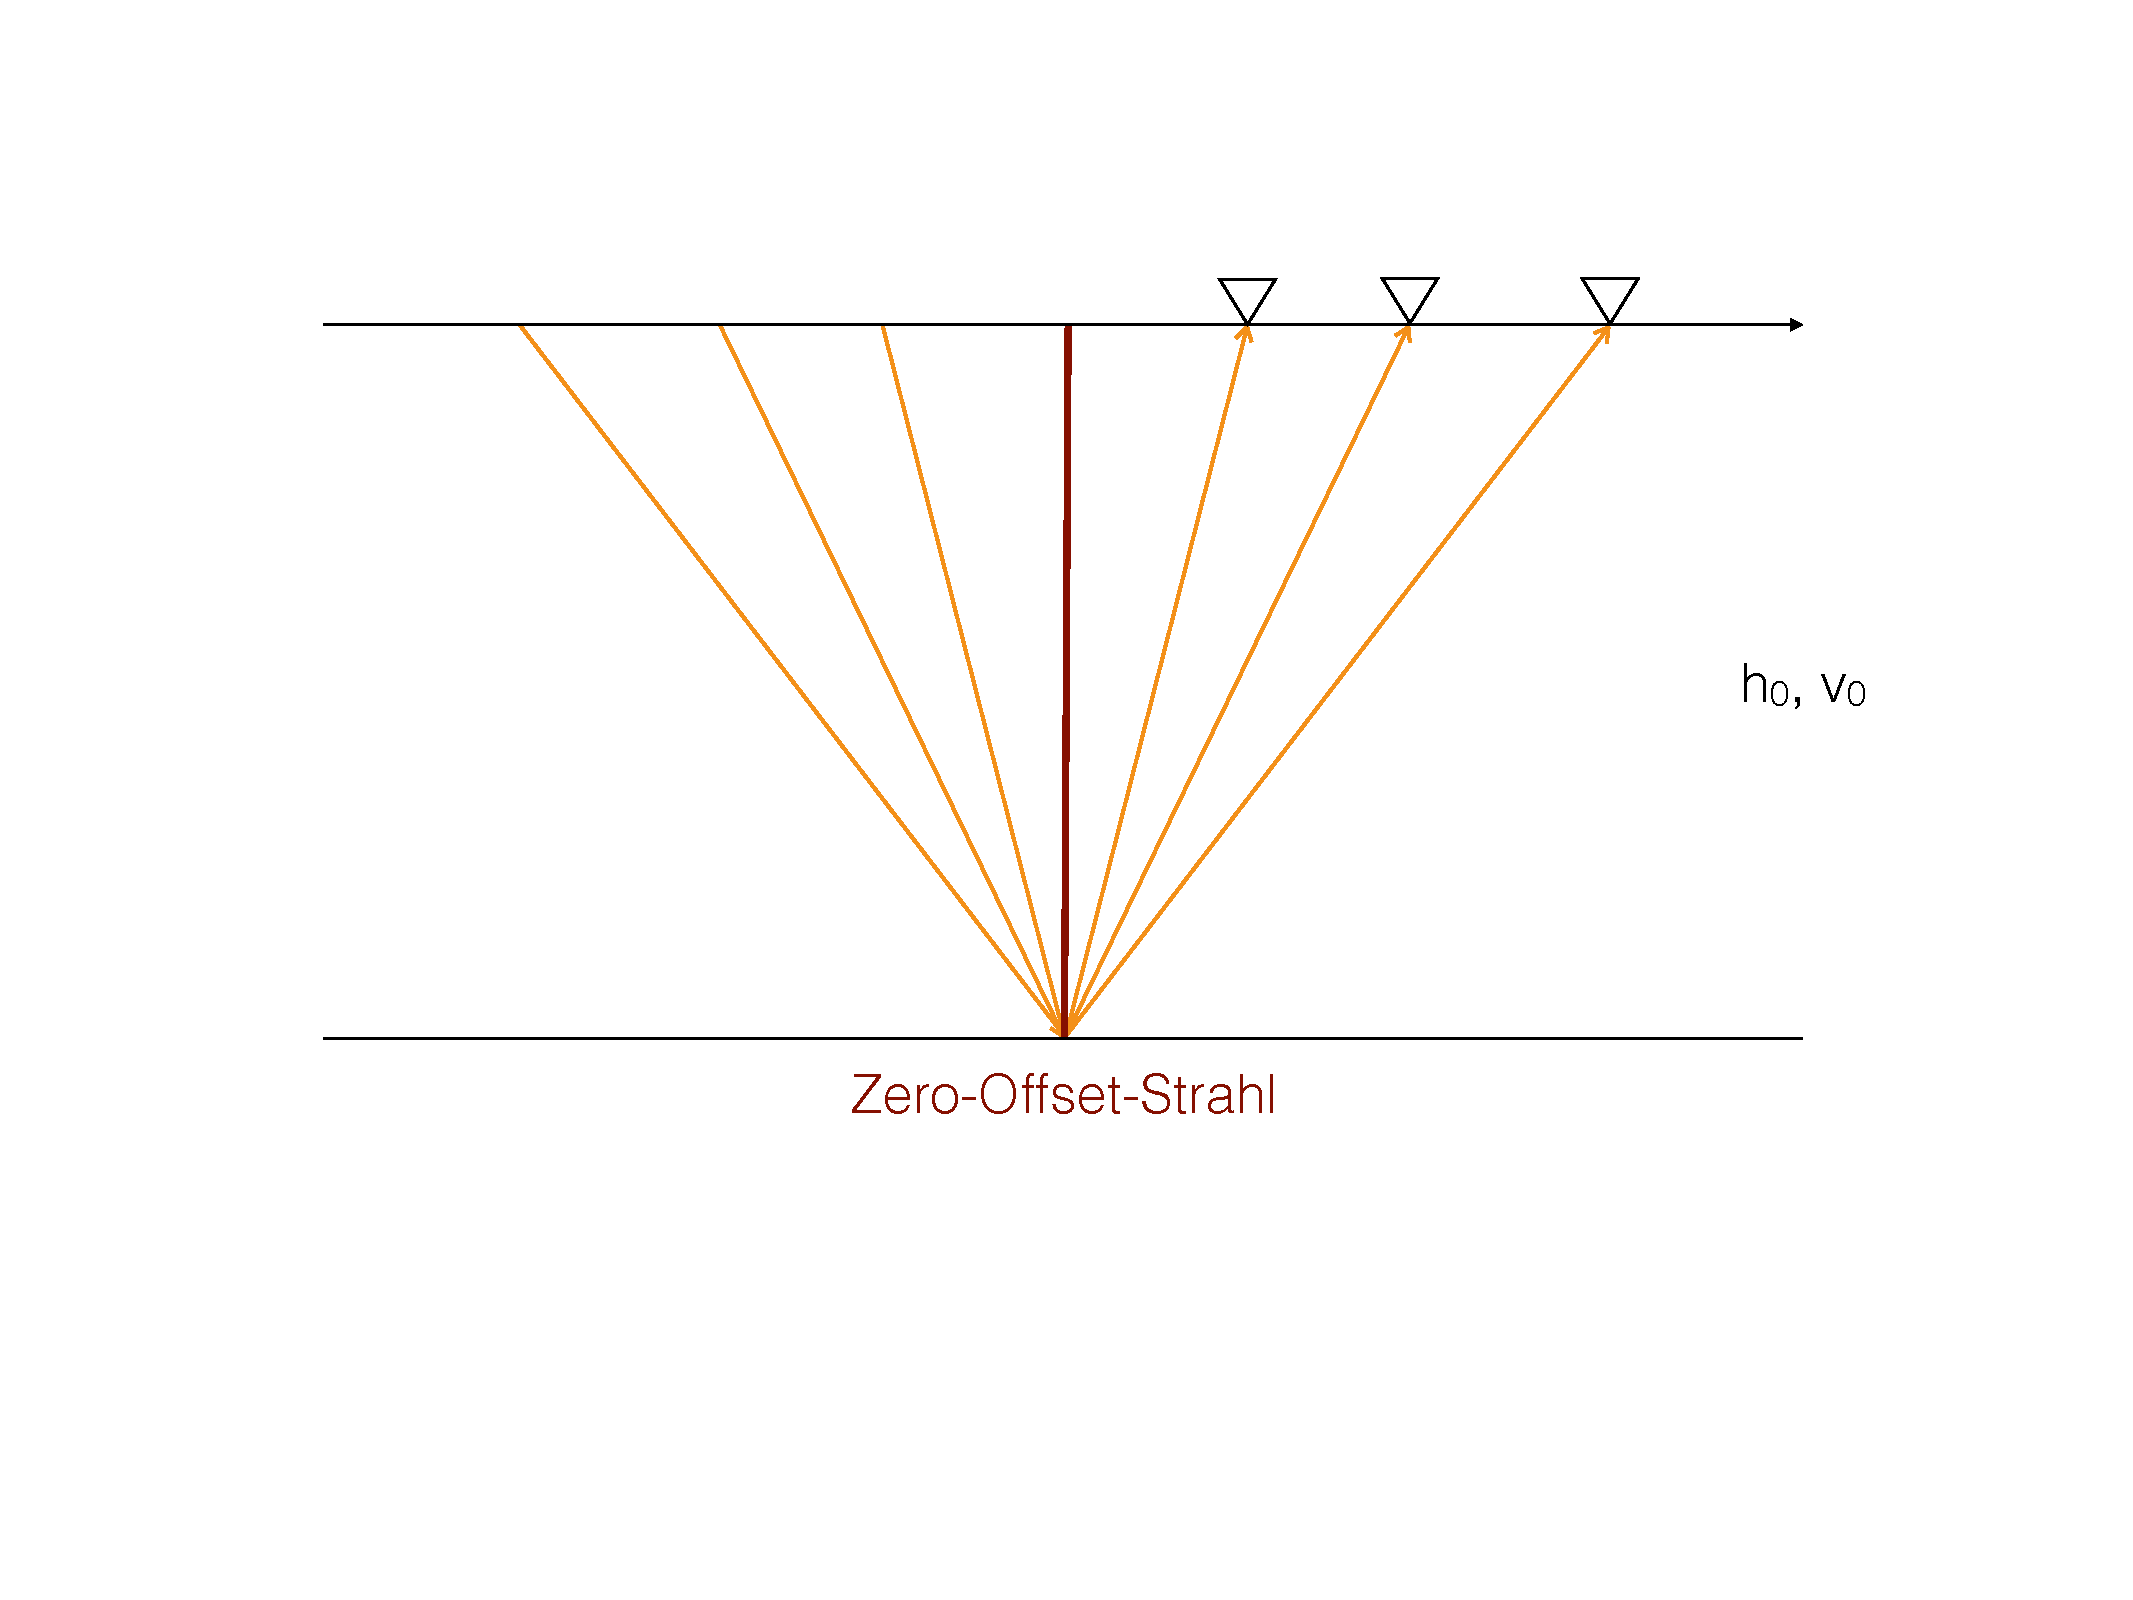
\includegraphics[width = \textwidth]{ReflexionsseismikBilder/ZeroOffsetStrahl}
\end{figure}

Betrachten wir erneut die Messauslage nach CMP-Sortierung und die zugehörige Laufzeitkurve: 

\begin{figure}[H]
	\begin{subfigure}[m]{0.5\textwidth}
	\centering
		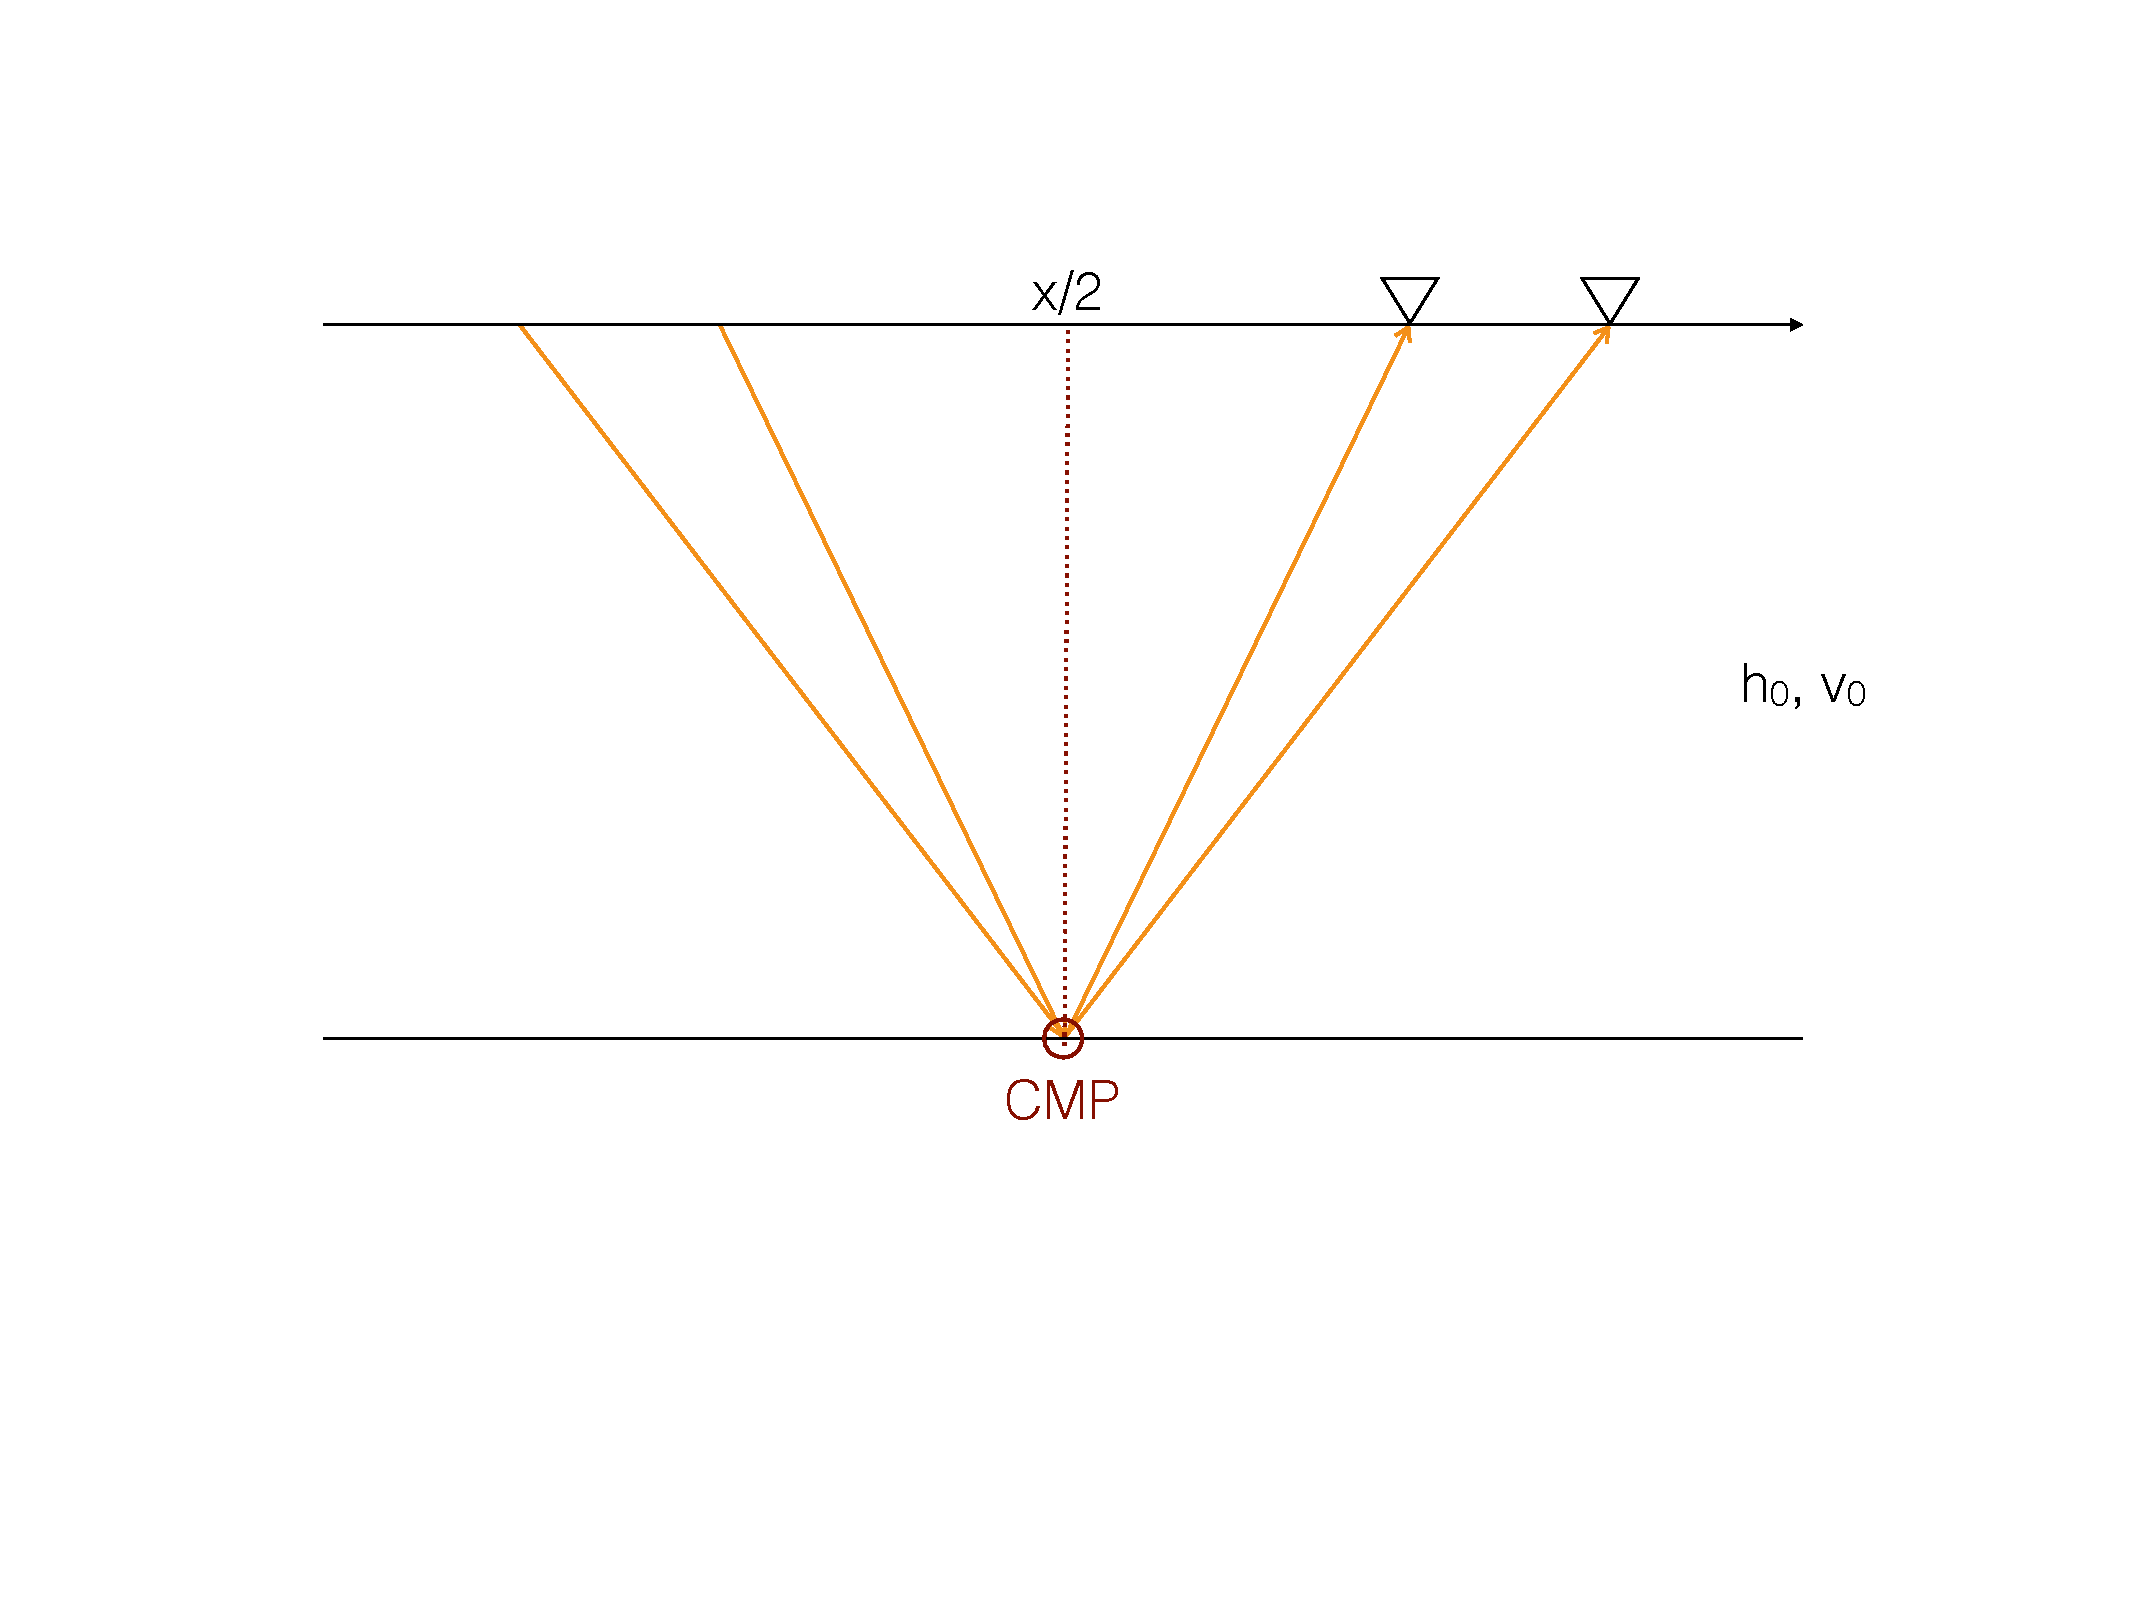
\includegraphics[scale = 0.2]{ReflexionsseismikBilder/CMPSortierung}	
	\end{subfigure}
	\begin{subfigure}[m]{0.5\textwidth}
	\centering
		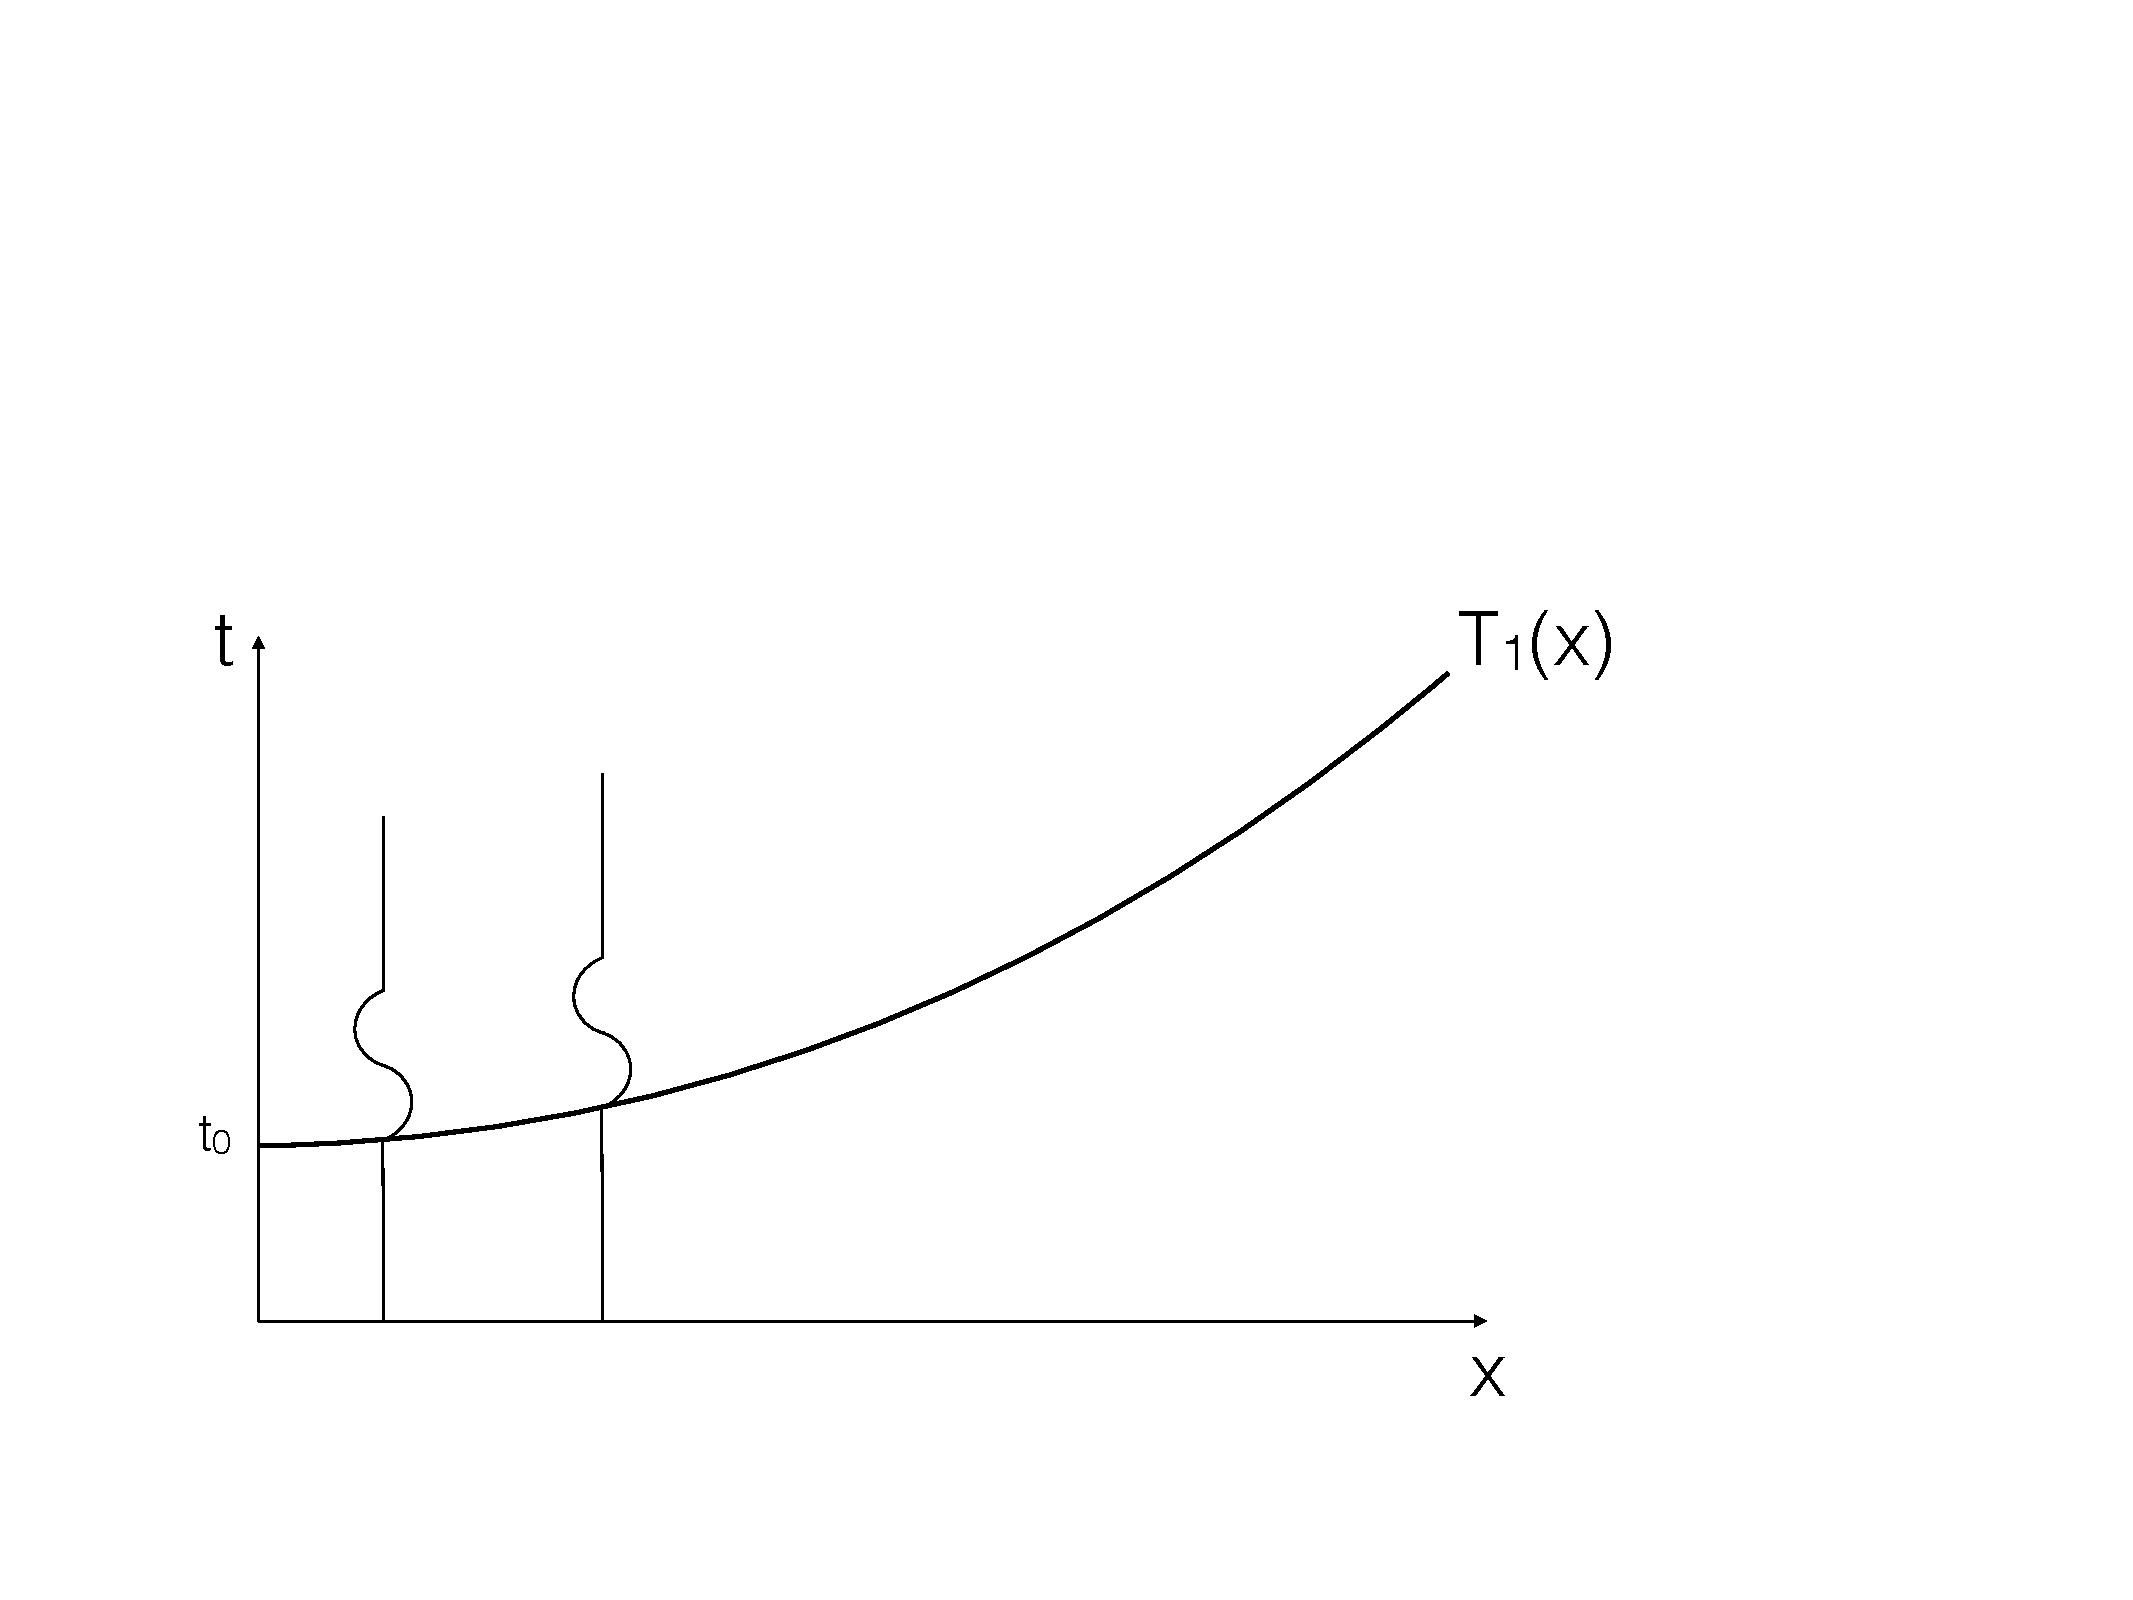
\includegraphics[scale = 0.2]{ReflexionsseismikBilder/LaufzeitCMP}
	\end{subfigure}
\end{figure}


Die Laufzeit der Welle mit dem kürzesten Weg ist genau $t_0$. Dieser Weg entspricht dem eines Zero-Offset-Strahls, also senkrecht nach unten und wieder nach oben.
Da die Wellen bei allen anderen Messauslagen einen größeren Weg zurücklegen müssen, ist die Laufzeitkurve eine Hyperbel und keine Gerade. Eine solche wollen wir aber erzeugen. Aus diesem Grund ist eine Laufzeitkorrektur durchzuführen. Diese Korrektur gleicht die längere Laufzeit, verursacht durch längere Strahlenwege, aus. 


\begin{equation*}
	\Delta t_{\text{nmo}} = T_1(x) - t_0 = \sqrt{\frac{x^2}{v_{\text{nmo}}^2} + t_0^2} - t_0
\end{equation*}   

\begin{figure}[H]
	\centering
	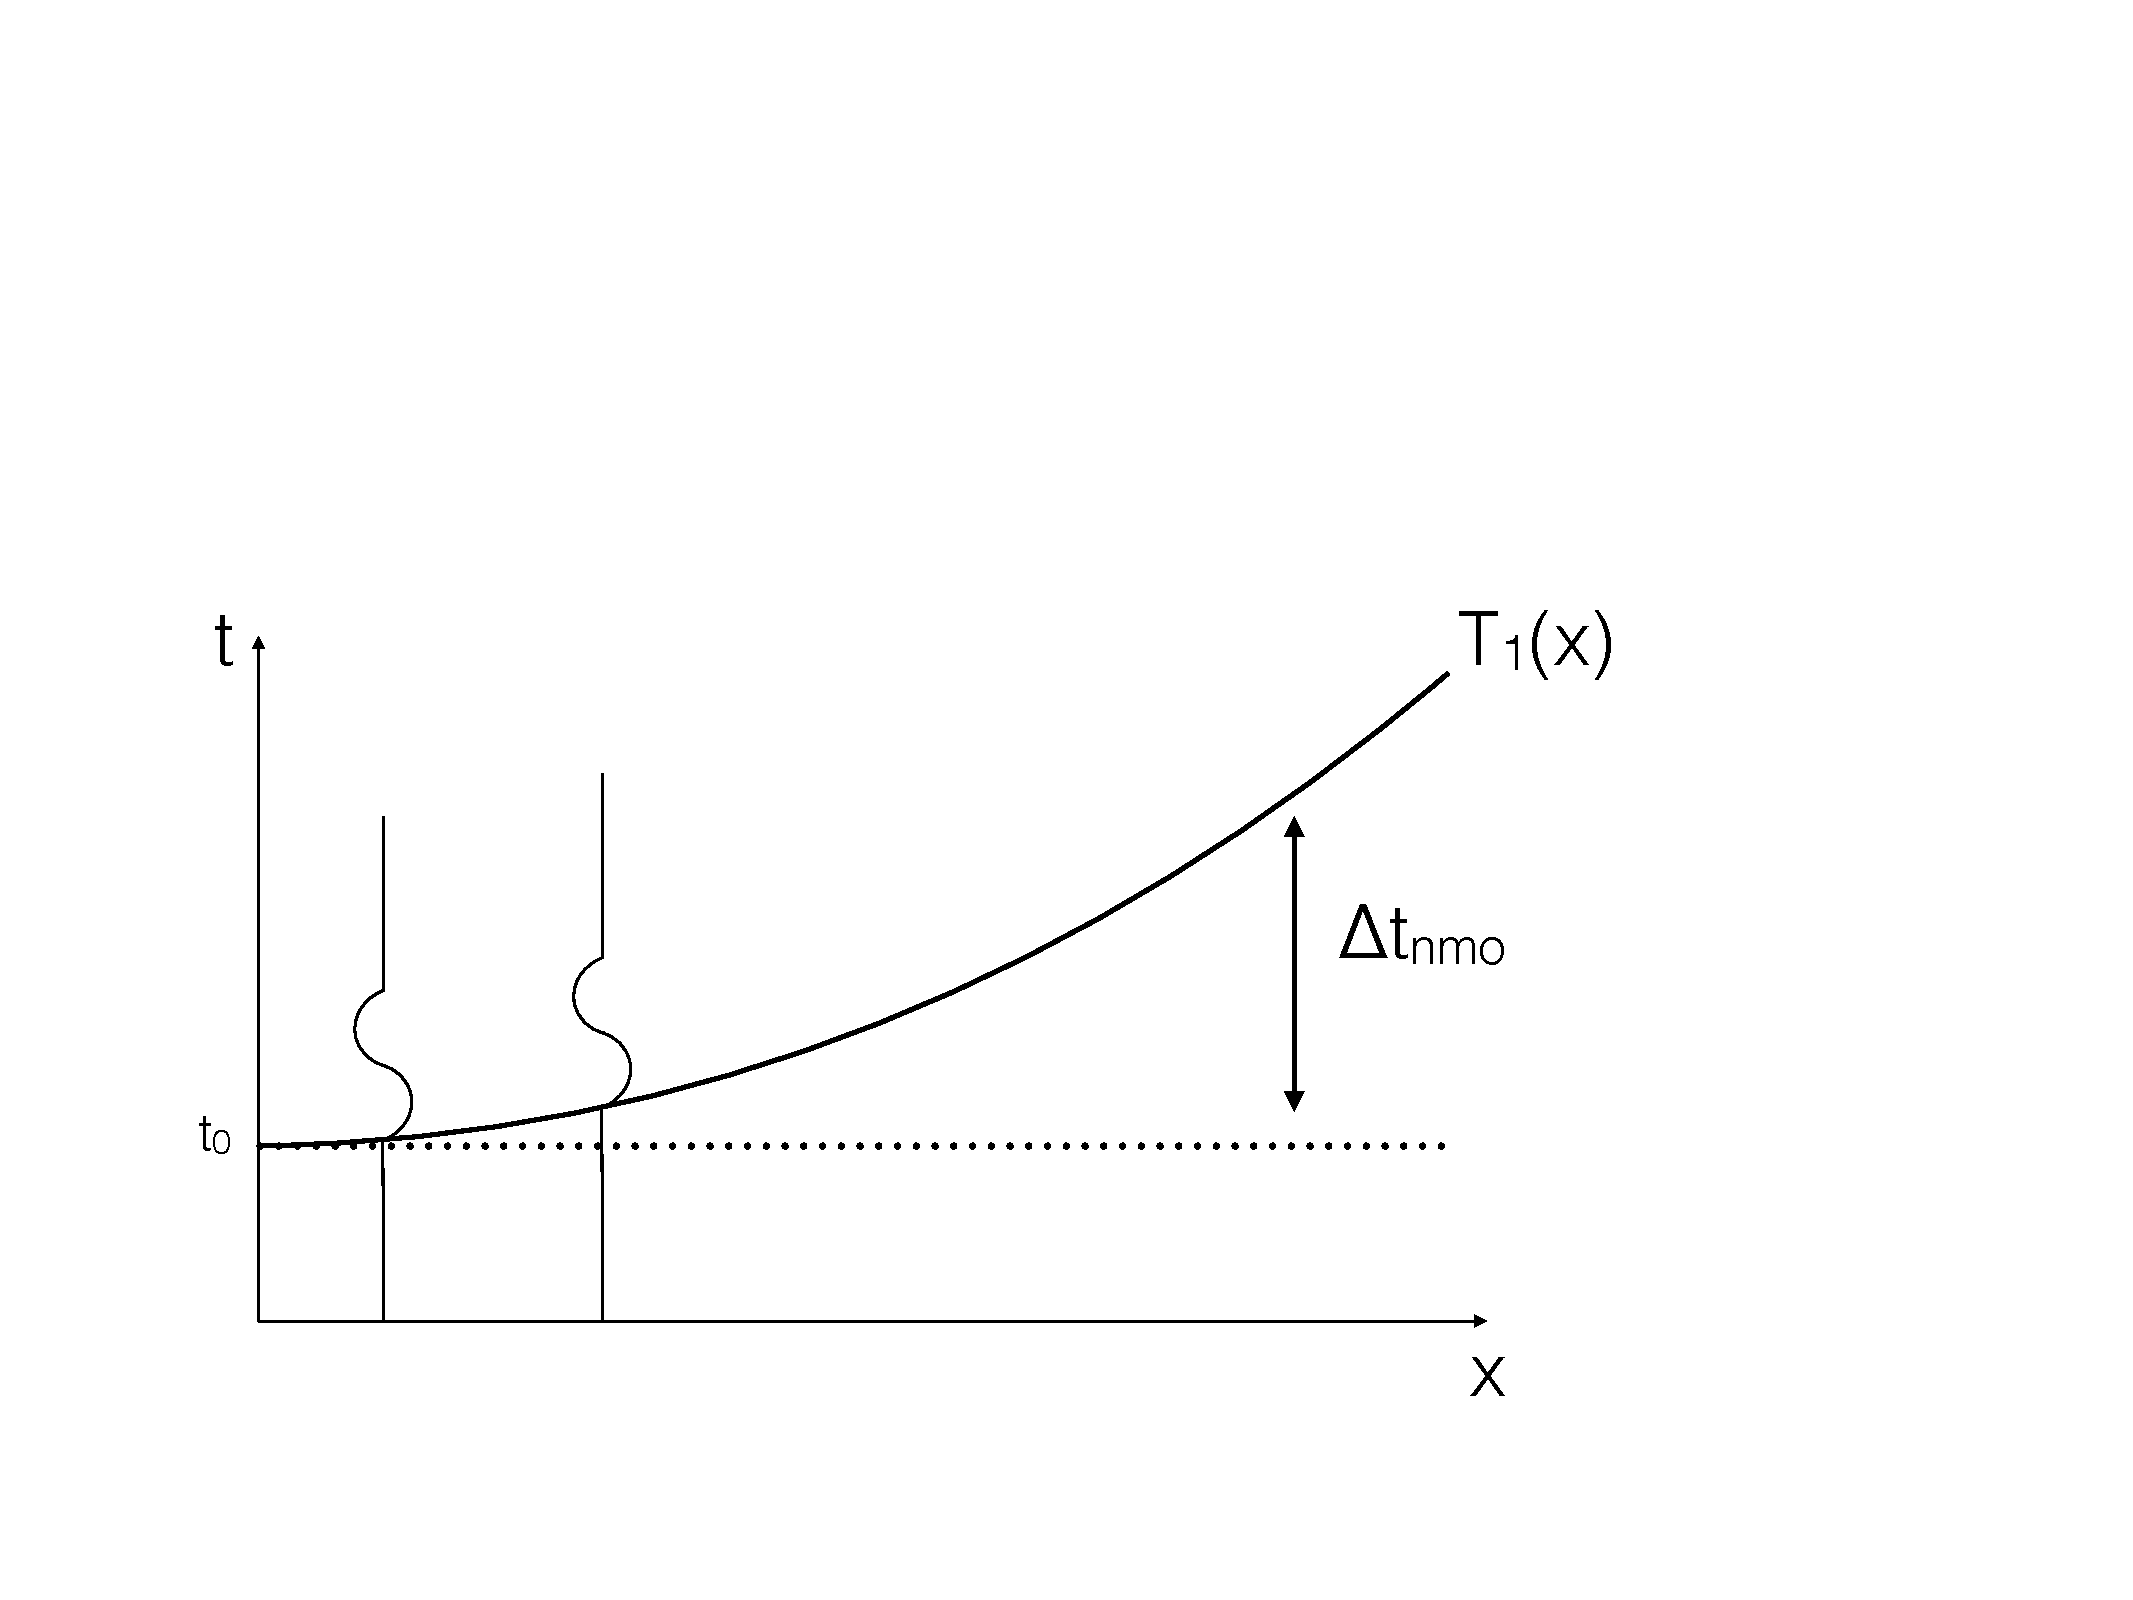
\includegraphics[scale = 0.3]{ReflexionsseismikBilder/tnmoAnpassung}
\end{figure}

\subsection{Stapelung}
Nachdem wir alle Messwerte auf eine Zeit normiert haben, werden die Seismogrammdaten gestapelt, das heißt aus allen Seismogrammen wird ein einziges pro CMP. Das Ergebnis ist ein Zero-Offset-Strahl ohne Mehrdeutigkeiten.

\begin{figure}[H]
	\centering
	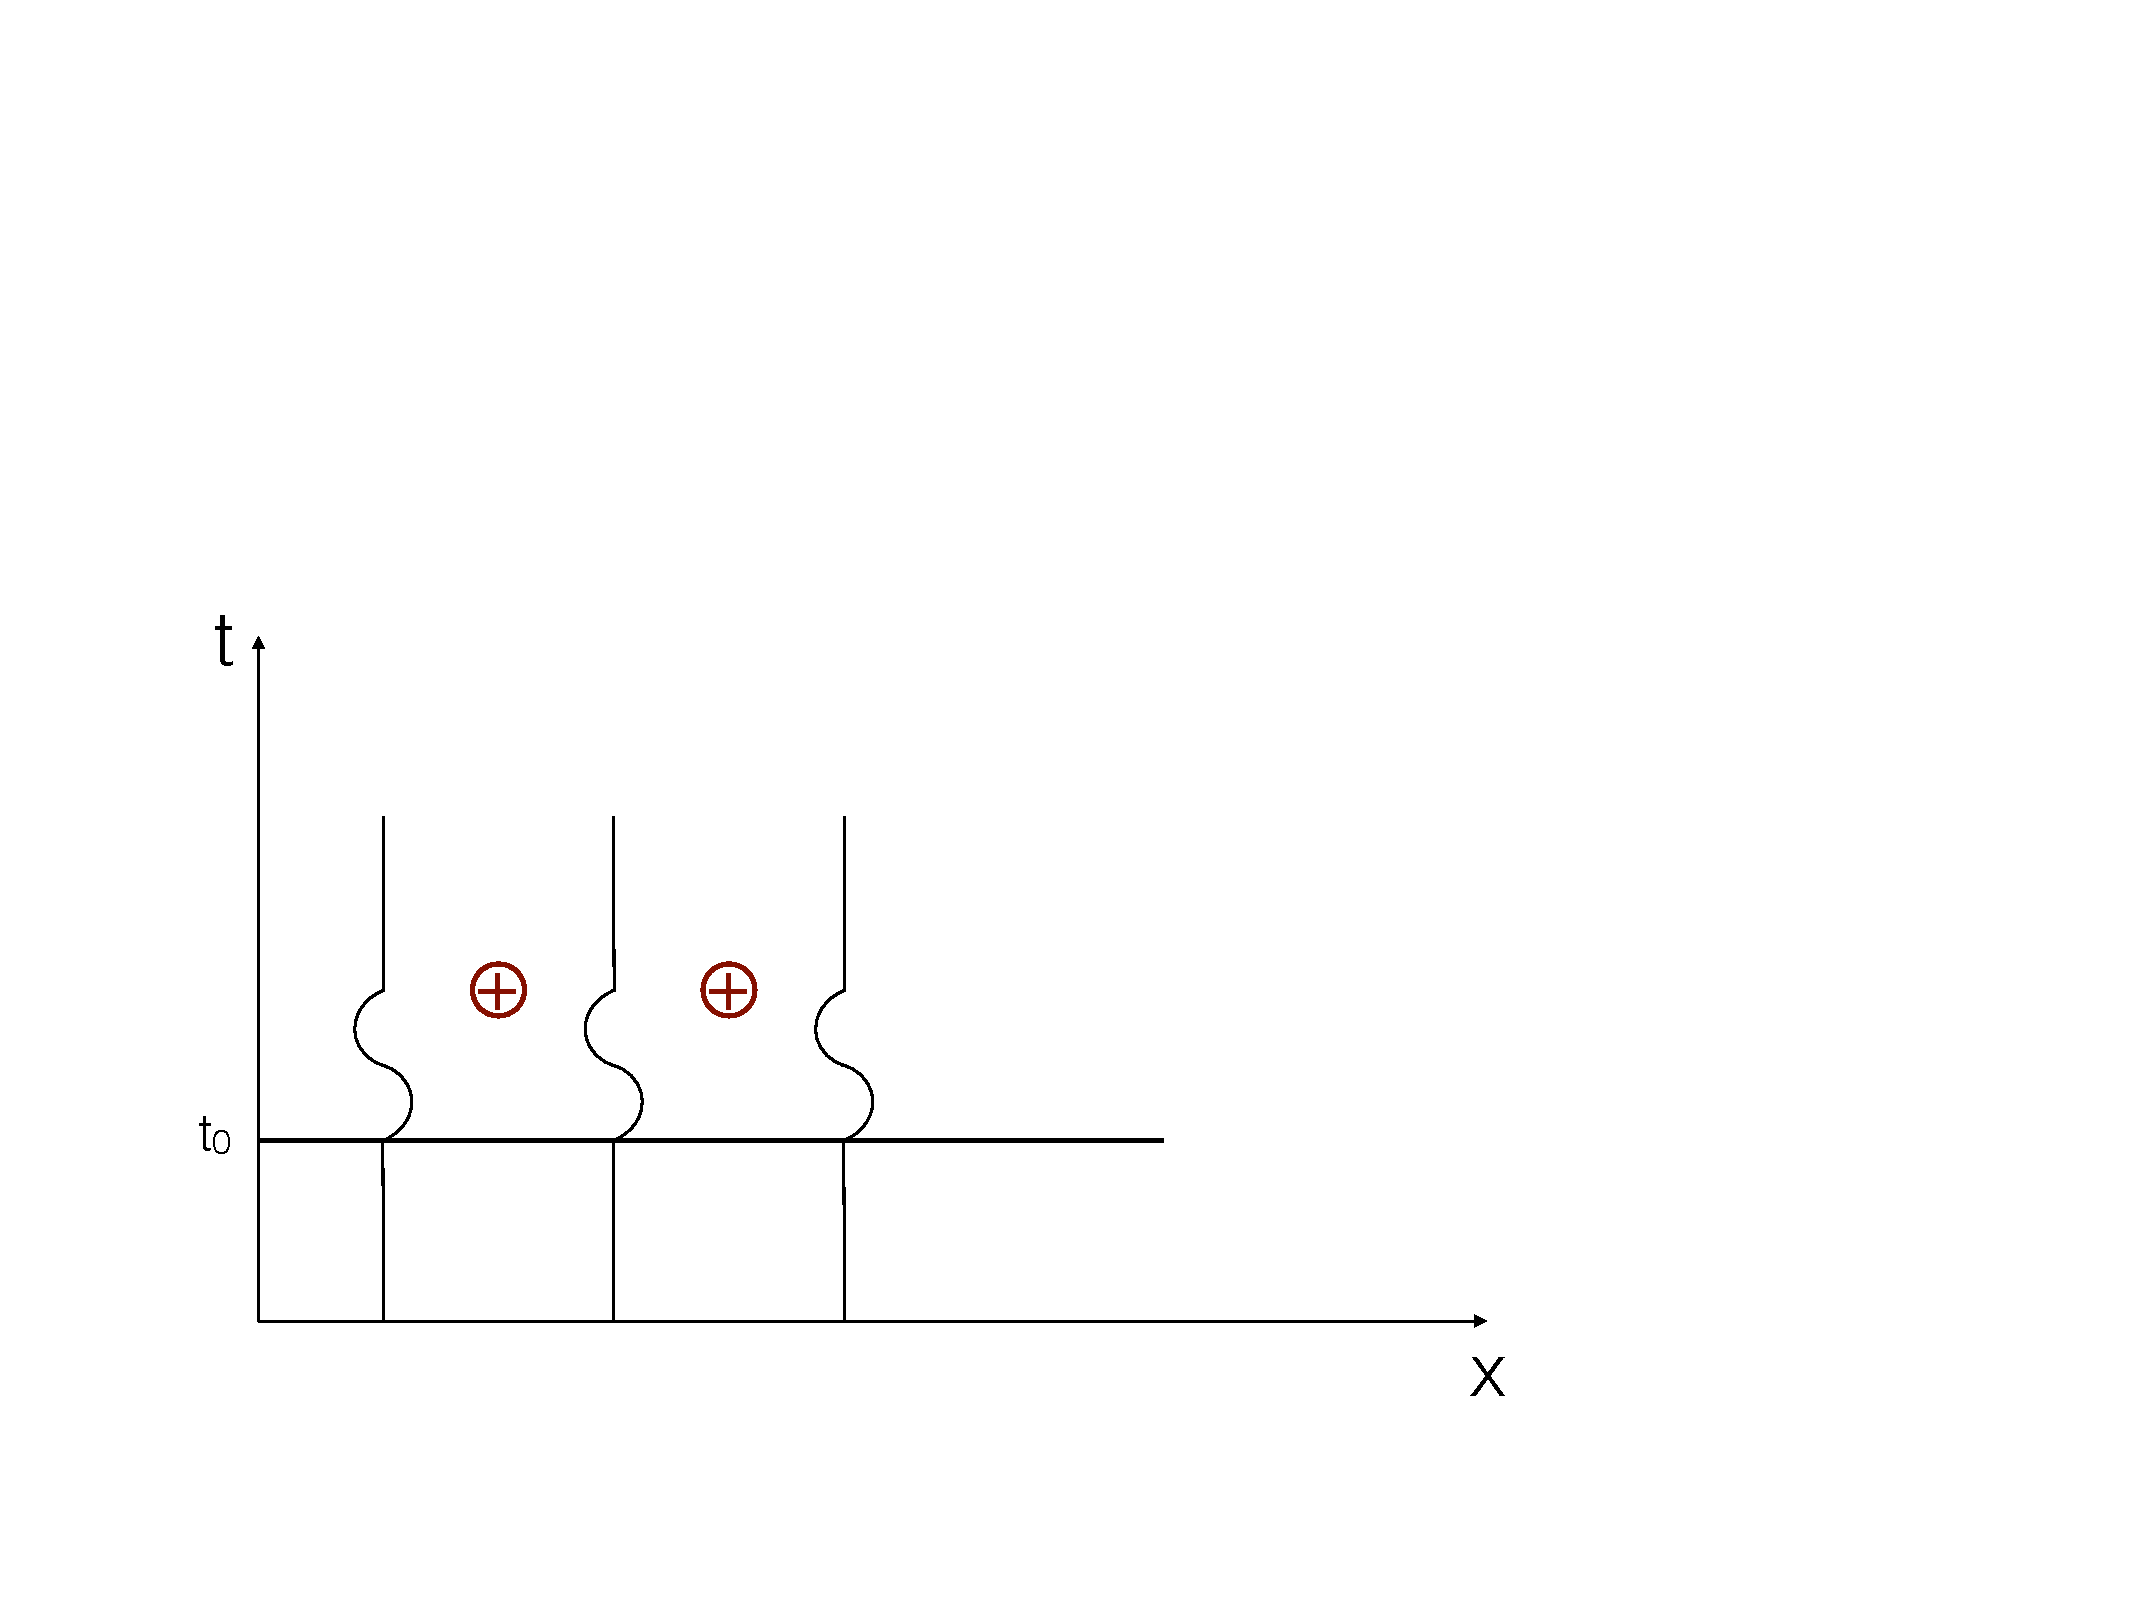
\includegraphics[width = \textwidth]{ReflexionsseismikBilder/Stapelung}
\end{figure}

\subsection{Berechnung der Schichtgeschwindigkeiten}

Trotz aller Maßnahmen zur Beseitigung der Mehrdeutigkeit ist unser Hauptziel noch nicht gelöst. Bisher haben wir nur die \textbf{Stapelgeschwindigkeiten} (Normal-Moveout-Geschwindigkeit) $v_{\text{nmo}}$, aber nicht die einzelnen \textbf{Intervallgeschwindigkeiten} $v_n$. Diese lassen sich jedoch einfach aus den Stapelgeschwindigkeiten berechnen. Der Zusammenhang wird durch die \textbf{Dix'sche Formel} beschrieben: \begin{equation*}
	v_n = \sqrt{\frac{v_{\text{nmo},n}^2 \cdot t_{0,n} - v_{\text{nmo},n-1}^2 \cdot t_{0,n-1}}{t_n - t_{n-1}}}
\end{equation*} 

 







